%%%%%%%%%%%%%%%%%%%%%%%%%%%%%%%%%%%%%%%%%%%%%%%%%%%%%%%%%%%%%%%
%% OXFORD THESIS TEMPLATE try

% Use this template to produce a standard thesis that meets the Oxford University requirements for DPhil submission
%
% Originally by Keith A. Gillow (gillow@maths.ox.ac.uk), 1997
% Modified by Sam Evans (sam@samuelevansresearch.org), 2007
% Modified by John McManigle (john@oxfordechoes.com), 2015
%
% This version Copyright (c) 2015-2017 John McManigle
%
% Broad permissions are granted to use, modify, and distribute this software
% as specified in the MIT License included in this distribution's LICENSE file.
%

% I've (John) tried to comment this file extensively, so read through it to see how to use the various options.  Remember
% that in LaTeX, any line starting with a % is NOT executed.  Several places below, you have a choice of which line to use
% out of multiple options (eg draft vs final, for PDF vs for binding, etc.)  When you pick one, add a % to the beginning of
% the lines you don't want.


%%%%% CHOOSE PAGE LAYOUT
% The most common choices should be below.  You can also do other things, like replacing "a4paper" with "letterpaper", etc.

% This one will format for two-sided binding (ie left and right pages have mirror margins; blank pages inserted where needed):
\documentclass[a4paper,twoside]{ociamthesis}
% This one will format for one-sided binding (ie left margin > right margin; no extra blank pages):
%\documentclass[a4paper]{ociamthesis}
% This one will format for PDF output (ie equal margins, no extra blank pages):
%\documentclass[a4paper,nobind]{ociamthesis} 
\usepackage[english, latin]{babel}
\usepackage[T1]{fontenc}
\usepackage[utf8]{inputenc}
\usepackage{csquotes}


%%%%% SELECT YOUR DRAFT OPTIONS
% Three options going on here; use in any combination.  But remember to turn the first two off before
% generating a PDF to send to the printer!

% This adds a "DRAFT" footer to every normal page.  (The first page of each chapter is not a "normal" page.)
\fancyfoot[C]{\emph{DRAFT Printed on  \today}}  

% This highlights (in blue) corrections marked with (for words) \mccorrect{blah} or (for whole
% paragraphs) \begin{mccorrection} . . . \end{mccorrection}.  This can be useful for sending a PDF of
% your corrected thesis to your examiners for review.  Turn it off, and the blue disappears.
\correctionstrue


%%%%% BIBLIOGRAPHY SETUP
% Note that your bibliography will require some tweaking depending on your department, preferred format, etc.
% The options included below are just very basic "sciencey" and "humanitiesey" options to get started.
% If you've not used LaTeX before, I recommend reading a little about biblatex/biber and getting started with it.
% If you're already a LaTeX pro and are used to natbib or something, modify as necessary.
% Either way, you'll have to choose and configure an appropriate bibliography format...

% The science-type option: numerical in-text citation with references in order of appearance.
\usepackage[style=numeric-comp, sorting=none, backend=bibtex, doi=false, isbn=false]{biblatex}
\newcommand*{\bibtitle}{References}
%backend=biber
% The humanities-type option: author-year in-text citation with an alphabetical works cited.
%\usepackage[style=authoryear, sorting=nyt, backend=biber, maxcitenames=2, useprefix, doi=false, isbn=false]{biblatex}
%\newcommand*{\bibtitle}{Works Cited}

% This makes the bibliography left-aligned (not 'justified') and slightly smaller font.
\renewcommand*{\bibfont}{\raggedright\small}

% Change this to the name of your .bib file (usually exported from a citation manager like Zotero or EndNote).
\addbibresource{references.bib}


% Uncomment this if you want equation numbers per section (2.3.12), instead of per chapter (2.18):
%\numberwithin{equation}{subsection}



%%%%% THESIS / TITLE PAGE INFORMATION
% Everybody needs to complete the following:
\title{Suitably impressive thesis title}
\author{Lennart Golks}
\college{Department of Physics}

% Master's candidates who require the alternate title page (with candidate number and word count)
% must also un-comment and complete the following three lines:
%\masterssubmissiontrue
%\candidateno{933516}
%\wordcount{28,815}

% Uncomment the following line if your degree also includes exams (eg most masters):
%\renewcommand{\submittedtext}{Submitted in partial completion of the}
% Your full degree name.  (But remember that DPhils aren't "in" anything.  They're just DPhils.)
\degree{Doctor of Philosophy}
% Term and year of submission, or date if your board requires (eg most masters)
\degreedate{November 2025}


%%%%% YOUR OWN PERSONAL MACROS
% This is a good place to dump your own LaTeX macros as they come up.

% To make text superscripts shortcuts
	\renewcommand{\th}{\textsuperscript{th}} % ex: I won 4\th place
	\newcommand{\nd}{\textsuperscript{nd}}
	\renewcommand{\st}{\textsuperscript{st}}
	\newcommand{\rd}{\textsuperscript{rd}}

\usepackage{amsmath, bm}
\usepackage{mathtools}
\usepackage{amsfonts}
\usepackage{cancel}
\usepackage{minitoc}
\usepackage{bookmark}
\usepackage{subfigure}


%%%%% THE ACTUAL DOCUMENT STARTS HERE
\begin{document}


%%%%% CHOOSE YOUR LINE SPACING HERE
% This is the official option.  Use it for your submission copy and library copy:
\setlength{\textbaselineskip}{22pt plus2pt}
% This is closer spacing (about 1.5-spaced) that you might prefer for your personal copies:
%\setlength{\textbaselineskip}{18pt plus2pt minus1pt}

% You can set the spacing here for the roman-numbered pages (acknowledgements, table of contents, etc.)
\setlength{\frontmatterbaselineskip}{17pt plus1pt minus1pt}

% Leave this line alone; it gets things started for the real document.
\setlength{\baselineskip}{\textbaselineskip}


%%%%% CHOOSE YOUR SECTION NUMBERING DEPTH HERE
% You have two choices.  First, how far down are sections numbered?  (Below that, they're named but
% don't get numbers.)  Second, what level of section appears in the table of contents?  These don't have
% to match: you can have numbered sections that don't show up in the ToC, or unnumbered sections that
% do.  Throughout, 0 = chapter; 1 = section; 2 = subsection; 3 = subsubsection, 4 = paragraph...

% The level that gets a number:
\setcounter{secnumdepth}{2}
% The level that shows up in the ToC:
\setcounter{tocdepth}{2}


%%%%% ABSTRACT SEPARATE
% This is used to create the separate, one-page abstract that you are required to hand into the Exam
% Schools.  You can comment it out to generate a PDF for printing or whatnot.
\begin{abstractseparate}
	Your abstract text goes here.  Check your departmental regulations, but generally this should be less than 300 words.  See the beginning of Chapter~\ref{ch:2-litreview} for more.


 % Create an abstract.tex file in the 'text' folder for your abstract.
\end{abstractseparate}


% JEM: Pages are roman numbered from here, though page numbers are invisible until ToC.  This is in
% keeping with most typesetting conventions.
\begin{romanpages}

% Title page is created here
\maketitle

%%%%% DEDICATION -- If you'd like one, un-comment the following.
%\begin{dedication}
%This thesis is dedicated to\\
%someone\\
%for some special reason\\
%\end{dedication}

%%%%% ACKNOWLEDGEMENTS -- Nothing to do here except comment out if you don't want it.
\begin{acknowledgements}
 	I acknowledge my heritage, the society I grew up in and my access to free education.
I feel very privileged. 
Without the support of my parents I would not be where I am
today, Dankesch{\"o}n! 
Danke Mama, Papa, Hinnerk, Jonna, Oma Sigrid und Mel. 
Shout out to all the friends I made along the way and for letting me chew your ear off about
all the issues I encountered.

Thank you, Colin Fox, for your support as a supervisor, your always honest feedback and almost never-ending knowledge. 
I also thank Annika Sepp{\"a}l{\"a}, and Harald Schwefel for the financial support of the first two years of my PhD and everyone who was involved in the CubeSat project.
Thanks to all the staff in the Department of Physics, Statistics, and Mathematics for guiding me through the storm of bureaucracy and helping me fill out the numerous forms for various things in the past few years.
%The education system i grew up in and the support of my parents and family.
%
%Personal, I would like to thank Alex Elliott for his wonderful help and support. None of this would be possible otherwise.
%
%
%
%

\end{acknowledgements}

%%%%% ABSTRACT -- Nothing to do here except comment out if you don't want it.
\begin{abstract}
	Your abstract text goes here.  Check your departmental regulations, but generally this should be less than 300 words.  See the beginning of Chapter~\ref{ch:2-litreview} for more.



\end{abstract}

%%%%% MINI TABLES
% This lays the groundwork for per-chapter, mini tables of contents.  Comment the following line
% (and remove \minitoc from the chapter files) if you don't want this.  Un-comment either of the
% next two lines if you want a per-chapter list of figures or tables.
%\dominitoc % include a mini table of contents
%\dominilof  % include a mini list of figures
%\dominilot  % include a mini list of tables

% This aligns the bottom of the text of each page.  It generally makes things look better.
\flushbottom

% This is where the whole-document ToC appears:
\tableofcontents

\listoffigures
	\mtcaddchapter
% \mtcaddchapter is needed when adding a non-chapter (but chapter-like) entity to avoid confusing minitoc

% Uncomment to generate a list of tables:
%\listoftables
%	\mtcaddchapter

%%%%% LIST OF ABBREVIATIONS
% This example includes a list of abbreviations.  Look at text/abbreviations.tex to see how that file is
% formatted.  The template can handle any kind of list though, so this might be a good place for a
% glossary, etc.

% database
\DTLnewdb{abbr}
%\DTLnewrow{abbr}\DTLnewdbentry{abbr}{label}{MRF}\DTLnewdbentry{abbr}{desc}{Markov Random Field}
%\DTLnewrow{abbr}\DTLnewdbentry{abbr}{label}{GMRF}\DTLnewdbentry{abbr}{desc}{Gaussian Markov Random Field}
%\DTLnewrow{abbr}\DTLnewdbentry{abbr}{label}{GOMOS}\DTLnewdbentry{abbr}{desc}{Global Ozone Monitoring by Occultation of Stars}
\DTLnewrow{abbr}\DTLnewdbentry{abbr}{label}{MCMC}\DTLnewdbentry{abbr}{desc}{Markov Chain Monte-Carlo}
\DTLnewrow{abbr}\DTLnewdbentry{abbr}{label}{RTE}\DTLnewdbentry{abbr}{desc}{Radiative Transfer Equation}
\DTLnewrow{abbr}\DTLnewdbentry{abbr}{label}{MLS}\DTLnewdbentry{abbr}{desc}{Microwave Limb Sounder}
\DTLnewrow{abbr}\DTLnewdbentry{abbr}{label}{NASA}\DTLnewdbentry{abbr}{desc}{National Aeronautics and Space Administration}
\DTLnewrow{abbr}\DTLnewdbentry{abbr}{label}{MTC}\DTLnewdbentry{abbr}{desc}{Marginal and then Conditional}
\DTLnewrow{abbr}\DTLnewdbentry{abbr}{label}{RMS}\DTLnewdbentry{abbr}{desc}{Root Mean Square}
\DTLnewrow{abbr}\DTLnewdbentry{abbr}{label}{STD}\DTLnewdbentry{abbr}{desc}{Standard Deviation}
%\DTLnewrow{abbr}\DTLnewdbentry{abbr}{label}{MVN}\DTLnewdbentry{abbr}{desc}{Multivariate Normal}
\DTLnewrow{abbr}\DTLnewdbentry{abbr}{label}{TT}\DTLnewdbentry{abbr}{desc}{Tensor-Train}
\DTLnewrow{abbr}\DTLnewdbentry{abbr}{label}{SIRT}\DTLnewdbentry{abbr}{desc}{Squared Inverse Rosenblatt Transform}
\DTLnewrow{abbr}\DTLnewdbentry{abbr}{label}{IRT}\DTLnewdbentry{abbr}{desc}{Inverse Rosenblatt Transform}
\DTLnewrow{abbr}\DTLnewdbentry{abbr}{label}{IACT}\DTLnewdbentry{abbr}{desc}{Integrated Autocorrelation Time}
\DTLnewrow{abbr}\DTLnewdbentry{abbr}{label}{MH}\DTLnewdbentry{abbr}{desc}{Metropolis--Hastings}
\DTLnewrow{abbr}\DTLnewdbentry{abbr}{label}{SVD}\DTLnewdbentry{abbr}{desc}{Singular Value Decomposition}
\DTLnewrow{abbr}\DTLnewdbentry{abbr}{label}{VMR}\DTLnewdbentry{abbr}{desc}{Volume Mixing Ratio}
\DTLnewrow{abbr}\DTLnewdbentry{abbr}{label}{HITRAN}\DTLnewdbentry{abbr}{desc}{High-Resolution Transmission}
\DTLnewrow{abbr}\DTLnewdbentry{abbr}{label}{DAG}\DTLnewdbentry{abbr}{desc}{Directed Acyclic Graph}
\DTLnewrow{abbr}\DTLnewdbentry{abbr}{label}{MWG}\DTLnewdbentry{abbr}{desc}{Metropolis within Gibbs}
%\DTLnewrow{abbr}\DTLnewdbentry{abbr}{label}{NL}\DTLnewdbentry{abbr}{desc}{Non-Linear}
\DTLnewrow{abbr}\DTLnewdbentry{abbr}{label}{L}\DTLnewdbentry{abbr}{desc}{Linear}
\DTLnewrow{abbr}\DTLnewdbentry{abbr}{label}{RTO}\DTLnewdbentry{abbr}{desc}{Randomise then Optimise}
\DTLnewrow{abbr}\DTLnewdbentry{abbr}{label}{CDF}\DTLnewdbentry{abbr}{desc}{Cumulative Distribution Function}
\DTLnewrow{abbr}\DTLnewdbentry{abbr}{label}{PDF}\DTLnewdbentry{abbr}{desc}{Probability Density Function}
\DTLnewrow{abbr}\DTLnewdbentry{abbr}{label}{MIPAS}\DTLnewdbentry{abbr}{desc}{Michelson Interferometer for Passive Atmospheric Sounding}
\DTLsort{label}{abbr}


\begin{mclistof}{List of Abbreviations}{4cm}
	\printmclist{abbr}
		\thispagestyle{empty}
\end{mclistof}
% First parameter can be changed eg to "Glossary" or something.
% Second parameter is the max length of bold terms.
%\begin{mclistof}{List of Abbreviations}{3.2cm}
%
%\item[i.i.d.]  independent and identically distributed
%
%\item[MRF] Markov Random Field
%
%\item[GMRF] Gaussian Markov Random Field
%
%\item[MTC] Marginal Then Conditional sampler
%
%\item[GOMOS] Global Ozone Monitoring by Occultation of Stars
%
%\item[MCMC] Markov Chain Monte-Carlo
%
%\item[MH] Metropolis-Hastings
%\end{mclistof} 
%\clearpage
%\begin{mclistof2}
%\item{label}{Banana}
%\item{label}{Apple}
%\item{label}{Cherry}
%\end{mclistof2} 
%\begin{sortedlist}{List of Abbreviations}{3.2cm}
%	
%	\sortitem[i.i.d.]  independent and identically distributed
%	
%	\sortitem[MRF] Markov Random Field
%	
%	\sortitem[GMRF] Gaussian Markov Random Field
%	
%	\sortitem[MTC] Marginal Then Conditional sampler
%	
%	\sortitem[GOMOS] Global Ozone Monitoring by Occultation of Stars
%	
%	\sortitem[MCMC] Markov Chain Monte-Carlo
%	
%	\sortitem[MH] Metropolis-Hastings
%
%\end{sortedlist} 
%\begin{sortedlist}
%%\sortitem[i.i.d.] independent and identically distributed
%%\sortitem[MRF]Markov Random Field
%
%\sortitem[GMRF]{Gaussian Markov Random Field}
%
%\sortitem[MTC]{Marginal Then Conditional sampler}
%%
%%\sortitem[GOMOS]{Global Ozone Monitoring by Occultation of Stars}
%%
%%\sortitem[MCMC]{Markov Chain Monte-Carlo}
%%
%%\sortitem[MH]{Metropolis-Hastings}
%
%\end{sortedlist}
%
%\nomenclature[x]{+x}{A special symbol.}
%\nomenclature{y}{Some letter.}
%\nomenclature{z}{The last letter.}
%\nomenclature{a}{The first letter.}
%\nomenclature{w}{Some other letter.}
%
%\printnomenclature

% The Roman pages, like the Roman Empire, must come to its inevitable close.
\end{romanpages}


%%%%% CHAPTERS
% Add or remove any chapters you'd like here, by file name (excluding '.tex'):
\flushbottom
\chapter{Introduction}

Here we briefly describe the standard currently used to retrieve atmospheric trace gas concentrations, e.g. ozone concentration, from limb-sounding measurements and what motivates us to employ a hierarchical Bayesian framework to address this inverse problem.
We explain how our approach contributes to and improves upon existing methods.
Lastly, we provide the reader with the thesis structure.


\section{Motivation}
Presently, the only operating ozone limb sounder is the Microwave Limb Sounder (MLS) on NASA's Aura satellite.
This satellite is gradually drifting away from its orbit and scheduled to be phased out by 2026~\cite{Bryan2024NASA}.
A group led by Harald Schwefel has proposed an alternative approach to fill this observational gap using a much smaller platform such as a 6U CubeSat (roughly $30\text{cm} \times 15\text{cm} \times 10\text{cm}$)~\cite{ustin2024current}. 
The proposed system includes a disk-shaped resonator targeting a narrow frequency band and converting the thermal radiation emitted by ozone molecules from the terahertz region to the optical domain~\cite{Suresh25,Sedlmeir14}. 
This frequency conversion offers a cost-effective and energy-efficient solution as it avoids the need for large, energy-hungry cooling devices that are traditionally required to capture terahertz signals. 
Instead, signal acquisition in the optical domain can be implemented by using compact, affordable, and low-power photonic technologies.

Currently, the inverse problem to retrieve any trace gas from limb-sounding data is approached by the atmospheric physics community using optimisation and regularisation techniques developed in the 1970s~\cite{rodgers1976retrieval, NASA2022MLSv5}.
These methods focus on finding the ``best fit to data but not the best fit to parameters''~\cite{tan2016LecNot}.
Instead, we employ a hierarchically structured Bayesian framework to provide a distribution of ozone profiles, which represents multiple possible solutions according to some given data.
This probabilistic approach allows us to determine meaningful estimates and uncertainties of parameters.

\section{Research Gap and Contribution}

As already mentioned, currently the MLS retrieval algorithm~\cite{livesey2006retrieval} is based on the ``optimal estimation'' method from~\cite{rodgers1976retrieval}.
This approach provides a point estimate by fitting parameters to some data and iteratively minimising a squared residual norm, penalised against a chosen regularisation.
However, this does not provide comprehensive information about the parameters' underlying correlation structures and can lead to unphysical results, e.g.~negative ozone concentration values~\cite{MLSdata}.
Additionally, the solutions may be biased and the bias is then removed based on empirical decisions~\cite{livesey2008ozonecarbonmono, Froidevaux2008snrozone}.
Errors are provided by a local derivative of the forward map at the optimal solution, which is inherently highly sensitive to that specific point in the parameter space.
Furthermore, these regularisation methods condition on external point estimates of other parameters such as temperature or pressure~\cite{livesey2006retrieval}.
%Recent machine learning efforts do not include noise as a retrieval hyper-parameter condition on one single noise value (point estimate) in the developed model, which is trained for about one month, and .
%Additionally they compare to a ``ground truth'' provided by the previously described optimal estimation approach \cite{werner2023machlearn, bojkov2008NeuralNet}.
%Recent machine learning approaches suffer from related limitations. These models are typically trained over short periods (e.g., one month), condition on a single fixed noise value, and do not treat noise as a retrieval hyper-parameter. Moreover, they are benchmarked against a “ground truth” derived from the same optimal estimation method described above~\cite{werner2023machlearn, bojkov2008NeuralNet}.

In the presence of measurement noise any observation process is a random process.
Consequently, in Bayesian modelling all unknown parameters are treated as random variables~\cite{kaipio2005statinv}.
Further, a hierarchically ordered model incorporates unknown hyper-parameters, which for example,~control the noise of the data and the smoothness of the ozone profile.
Therefore, it is able to model conditional dependencies between parameters and hyper-parameters.
For some given data, the posterior probability distribution of this hierarchical Bayesian framework provides a range of feasible unbiased solutions and hence true errors.
Livesey et al.~\cite{livesey2006retrieval} report ``unexpected spectrally correlated noise'' on the MLS Aura, so here is another real reason why one should include noise in the model.

In this thesis, the marginal and then conditional (MTC) method~\cite{fox2016fast} is utilised and a hierarchical Bayesian model based on the radiative transfer equation (RTE) is developed.
First, the non-linearity of the RTE is neglected and a linear-Gaussian hierarchical Bayesian model is employed to provide a posterior distribution of ozone profiles.
Since the RTE is weakly non-linear we use the previously obtained results to find an affine map that approximates the non-linear forward model.
This appears to be a novelty in the field of atmospheric remote sensing.
Lastly, the hierarchical Bayesian framework is extended to jointly infer ozone, pressure and temperature.
The MTC scheme is a relatively new method within the Bayesian community, and we are the first, to the best of our knowledge, to apply it to a forward model based on the RTE and to jointly provide posterior ozone, pressure, and temperature profiles.

Usually sampling algorithms are used to characterise the posterior probability distribution of a hierarchical Bayesian model. Instead, we approximate the posterior distribution directly utilising the tensor-train (TT) format~\cite{cui2022deep}. 
This allows us to generate independent samples from a TT approximation via a scheme similar to the inverse Rosenblatt transform (IRT)~\cite{dolgov2020approximation} with far fewer function evaluations compared to conventional samplers.
Further, in the TT format one can calculate marginal probability distributions of each hyper-parameter and evaluate integrals via quadrature without any sampling.


%and first the treat the 
%to solve this inverse problem and employ a linear-Gaussian hierarchical Bayesian framework.
%Within seconds we can evaluate the marginal posterior distribution over the hyper-parameters and the conditional posterior distribution over the parameters. \textcolor{red}{this does not clearly say that you treat a nonliner problem later.}
%This is a relatively new method within the Bayesian community, and is the first application to a forward model based on the radiative transfer equation (RTE), to the best of our knowledge. \textcolor{red}{already too many "we". Try something like : the sthe application in this thesis is ... the fist, to the besy of our knowledge.}
%
%
%This means that noise is controlled by a hyperparameter and included in the model as well as other hypeparaemntes and ozone as a paramtere.
%Since we deal with random varaibel described by distributions we provide posterior distribution of variabel which all present feasible solution to the data instead of on ``optimal'' solution.
%
%Naturally, noise (hyper-parameter) is a random process and follows a probability distribution, which we assume to know.
%According to that noise, as well as some other probability distributions, we can formulate explicit functions over hyper-parameters and parameters (e.g. ozone concentrations).\textcolor{red}{why is this here -- not clear to me}
%By incorporating hyper-parameters, e.g. measurement noise and smoothness of the ozone profile, in the modelling and inversion process, we are able to provide errors and a range of feasible paramters (posterior distribution) given some data, instead of one ``optimal'' solution.\textcolor{red}{ what kind of functions - -presently I can't work out what this says}
%This approach is known as hierarchical Bayesian modelling.\textcolor{red}{  OH, your trying to say that a hyperparametr controls something about the distribution of the noise, not that the noise is a hyperparameter, which is how this sentence reads.}
%\textcolor{red}{likewise. Besides, this sentence is not true. You know about the Approximation and Sampling paper.}
\section{Thesis Structure}
\begin{itemize}
	\item In Chapter~\ref{ch:background}, a brief introduction to hierarchical Bayesian modelling, sample-based estimates, TT approximations and regularisation approaches is given. We provide some background information along with references for further reading.
	\item Chapter~\ref{ch:formodel} introduces the simplified forward model based on the RTE following the Michelson interferometer for passive atmospheric sounding (MIPAS).
	We simulate data based on a ground truth and explain the process of doing so.
	Five different ways to acquire data are tested, and a singular value decomposition (SVD) of the forward model is performed to assess its information content.
	Given the SVD of the test cases, the most effective measurement method is determined.
	\item In Chapter~\ref{ch:LinVsReg}, the problem is treated as a linear inverse problem by neglecting the absorption term in the RTE. Some prior modelling aspects are discussed, and a linear-Gaussian hierarchical Bayesian model is established.
	Within the MTC scheme the marginal posterior over the hyper-parameters is evaluated first and then the full conditional posterior for ozone.
	Here, the marginal posterior is approximated in the TT format and the TT approximation is compared to sample-based results.
	Then posterior ozone profiles and a regularised estimate are compared to the ground truth.
	The chosen regularisation framework is the closest equivalent to the hierarchical Bayesian model in this Chapter.
	\item In Chapter~\ref{ch:affine}, the previously obtained posterior ozone profiles are used to find an affine map that approximates the non-linear RTE. The hierarchical Bayesian model from Chapter~\ref{ch:LinVsReg}, but with the approximate forward model, is used to obtain the posterior distribution of ozone profiles via the MTC scheme.
	\item In Chapter~\ref{ch:FullBay}, we extend the hierarchical Bayesian model to include pressure and temperature-related hyper-parameters.
	Prior modelling choices are discussed and the MTC method is utilised to obtain the marginal posterior over the hyper-parameters first and then the full conditional posterior of ozone.
	The reader is guided through the process of setting up an efficient 18-dimensional TT approximation of the marginal posterior.
	Some important aspects for improving the effectiveness and stability of TT approximations are highlighted.
	The TT approximation is compared to the results of the t-walk sampler on the marginal posterior.
	Posterior pressure and temperature profiles are obtained by sampling from the marginal posterior.
	Ozone samples of the full conditional posterior are drawn via the randomise then optimise method.
	\item In Chapter~\ref{ch:Concl}, some of the key differences between a regularisation approach and a hierarchical Bayesian approach are pointed out. Further, the advantages and disadvantages of TT approximations compared to conventional sampling methods are discussed.
	Lastly, we situate our results in the context of atmospheric physics and provide an outlook for future work.
\end{itemize}
All programming and analysis in this thesis are done in Python, and the reported computation times are taken on a MacBook Pro from 2019 with a 2.4 GHz quad-core Intel i5 processor.
% \begin{savequote}[8cm]
% Alles Gescheite ist schon gedacht worden.\\
% Man muss nur versuchen, es noch einmal zu denken.

% All intelligent thoughts have already been thought;\\
% what is necessary is only to try to think them again.
%   \qauthor{--- Johann Wolfgang von Goethe \cite{von_goethe_wilhelm_1829}}
% \end{savequote}



%\minitoc

%\section{Introduction}



% We define the probability density function (pdf) for a normally distributed random variable $x$ as:

% \begin{equation}
%     f(x; \mu, \sigma^2 ) = \frac{1}{\sigma \sqrt{2 \pi}} \exp{\Bigg[ - \frac{( x - \mu )^2}{2 \sigma^2} \Bigg] }  \tag{$-\infty < x < \infty, -\infty < \mu < \infty, \sigma > 0$}
% \end{equation}
% Here $\mu$ represents the mean, $\sigma^2$ the variance and $\sigma$ the standard deviation of the normal distribution $f(x)$ \cite{patel1996handbook}.
% If we describe $n$ normally distributed random variables, we do this with a multivariate Gaussian:
% \begin{equation}
%     \mathbf{x} = \begin{bmatrix}
%            x_{1} \\
%            \vdots \\ 
%            x_{n}
%          \end{bmatrix} 
%          \sim 
%          \mathcal{N}\begin{pmatrix} 
%          \begin{bmatrix}
%            \mu_{1} \\
%            \vdots \\ 
%            \mu_{n}
%          \end{bmatrix}
%          ,
%          \bm{\Sigma}
%          \end{pmatrix},
% \end{equation}
% where each normally distributed variable $x_i$ with $i = (1 \cdots n)$ has a mean $\mu_i$ and a variance... .
% The inverse of the variance is the precision matrix $\bm{\Sigma}^{-1} = \bm{Q}$
% \begin{align}
%     \pi( \bm{x} ) &= \pi(x_1) \pi(x_2 | x_1) \cdots \pi(x_n | x_{n-1} ) \\
%     &= \frac{1}{(2 \pi)^{n/2}} |\bm{Q}|^{1/2} \ \, \exp{\Bigg[ - \frac{1}{2} \bm{x}^T \bm{Q} \bm{x} \Bigg]} \\ 
%      &= \frac{1}{(2 \pi)^{n/2}} |\bm{\Sigma}|^{-1/2} \exp{\Bigg[ - \frac{1}{2} \bm{x}^T \bm{\Sigma}^{-1} \bm{x} \Bigg]}
% \end{align}

% \begin{equation}
%     \begin{bmatrix}
%            x_{1} \\
%            x_{2}
%          \end{bmatrix} 
%          \sim 
%          \mathcal{N}\begin{pmatrix} 
%          \begin{bmatrix}
%            \mu_{1} \\
%            \mu_{2}
%          \end{bmatrix}
%          ,
%          \begin{bmatrix}
%              \bm{\Sigma}_{11} & \bm{\Sigma}_{12}\\
%              \bm{\Sigma}_{21} & \bm{\Sigma}_{22}
%          \end{bmatrix}
%          \end{pmatrix}
% \end{equation}

% \begin{equation}
%     \begin{bmatrix}
%            x_{1} \\
%            x_{2}
%          \end{bmatrix} 
%          \sim 
%          \mathcal{N}\begin{pmatrix} 
%          \begin{bmatrix}
%            \mu_{1} \\
%            \mu_{2}
%          \end{bmatrix}
%          ,
%         \bm{Q}^{-1}
%          \end{pmatrix}
% \end{equation}

% \begin{align}
% \ln{\pi(\bm{x|y})} =& \ln{\pi( \bm{x} ) } + \ln{ \pi( \bm{y} | \bm{x} ) } \\
% =& - \frac{1}{2} (\bm{x} - \bm{\mu} )^T \bm{Q_x} (\bm{x} - \bm{\mu} ) - \frac{1}{2} (\bm{y} - \bm{Ax} )^T \bm{Q_x} (\bm{y} - \bm{Ax} )    \\
% =& - \frac{1}{2} \bigg[ \bm{x}^T \big[ \bm{Q_x} + \bm{A}^T \bm{Q_y} \bm{A} \big] \bm{x}  + \bm{x}^T \big[ - \bm{A}^T \bm{Q_y} \big] \bm{y} \\
% &+ \bm{y}^T \big[ - \bm{Q_y A} \big] \bm{x} + \bm{y}^T \big[ \bm{Q_y} \big] \bm{y} - 2 \bm{x}^T \bm{Q_x \mu }  \bigg] + \text{const.}
% \end{align}

% \begin{align}
%     &- \frac{1}{2} \begin{bmatrix}
%         \bm{x}^T \big[ \bm{Q_x} + \bm{A}^T \bm{Q_y} \bm{A} \big]  + \bm{y}^T \big[ - \bm{Q_y A} \big] & \bm{y}^T \big[ \bm{Q_y} \big] + \bm{x}^T \big[ - \bm{A}^T \bm{Q_y} \big] 
%     \end{bmatrix}  \begin{bmatrix}
%         \bm{x} \\ \bm{y}
%     \end{bmatrix} \\
%     =& \begin{bmatrix}
%         \bm{x}^T & \bm{y}^T
%     \end{bmatrix} 
%     \underbrace{\begin{bmatrix}
%         \bm{Q}_x + \bm{F}^T \bm{Q}_y \bm{F} & - \bm{F}^T \bm{Q}_y \\
%         -\bm{Q}_y \bm{F} & \bm{Q}_y
%     \end{bmatrix}}_\text{precision matrix} \begin{bmatrix}
%         \bm{x} \\ \bm{y}
%     \end{bmatrix} 
% \end{align}


% \begin{align}
%     \frac{- 2 \bm{x}^T \bm{Q_x \mu } }{-2} = \begin{bmatrix}
%         \bm{x}^T & 0
%     \end{bmatrix} \begin{bmatrix}
%         \bm{Q_x \mu}\\ 0
%     \end{bmatrix} \\
%     \Rightarrow \bm{\mu} = \bm{Q}^{-1} =  \begin{bmatrix}
%         \bm{Q_x \mu}\\ 0
%     \end{bmatrix}
% \end{align}
% \begin{equation}
%     \bm{Q} = \begin{bmatrix}
%         \bm{Q}_x + \bm{F}^T \bm{Q}_y \bm{F} & - \bm{F}^T \bm{Q}_y \\
%         -\bm{Q}_y \bm{F} & \bm{Q}_y
%     \end{bmatrix}
% \end{equation}









% \begin{subequations}
% \begin{align}
%     \bm{x|y, \theta} &\sim \mathcal{N}(\bm{F x}, \bm{Q_y}(\bm{\theta})) \quad \, \text{(likelihood)}\\
%     \bm{x| \theta} &\sim \mathcal{N}(\bm{\mu}, \bm{Q_x}(\bm{\theta})) \qquad \text{(prior)} \\
%     \bm{\theta} &\sim \pi(\bm{\theta}) \qquad \qquad \qquad \! \text{(hyperprior)}
% \end{align}
% \end{subequations}


% % \cite{simpson2012think}



% %\section{Gaussian Markov Random Fields}
% specify locally
% model globally
% set of RV

\chapter{\label{ch:2-litreview}Background}
This chapter provides the background knowledge for the applied methods.
We try to carefully guide the reader through the various topics so that we build a base to understand the used methodology.
Firstly, we discuss Markov Random Fields and their key properties to describe spatially connected variables in Section \ref{subsec:MRF}.
In Section \ref{subsec:NormDist} we introduce the normal distribution to describe the random variables in such a field.
By specifying the local connections in Section \ref{subsec:SpatialDepend} we globally observe a Gaussian Markov Random Field (GMRF).
Next, in Section \ref{sec:Bayesian} we relate the variables in the GMRF to a measurement process through a Bayesian Model.
Given the measurement, we try to find the most likely variables through a Markov chain, as described in Section \ref{subsec:Markov}.
Constructing this Markov chain we present the Metropolis-Hastings algorithm in Section \ref{subsec:MetroHast}, followed by the Marginal and then conditional sampler in Section \ref{subsec:MTC} and the adaptive Metropolis-Hastings algorithm in Section \ref{subsec:GOMOS}. 



\section{Gaussian Markov Random Field}
In this section, we guide the reader through the basic principles of Gaussian Markov Random Fields (GMRF).
We discuss some of the key properties of GMRFs and how to set up such a spatial field.
The discussed topics are strongly related to our specific application and for further reading, we refer to the books \cite{rue2005gaussian, higdon2006primer}.

\subsection{Markov Random Field}
\label{subsec:MRF}
A Markov Random Field (MRF) is based on a graphical model describing spatial dependencies of $n$ nodes, also described as vertices.
We label each node with an integer $i$ and attach a spatial position $s^{(i)}$ and a random variable $x^{(i)}$, where $i = 1, \dots, n$.
On a set of all vertices $\mathcal{V}$ we define an undirected graph $\mathcal{G}(\mathcal{V},\mathcal{E})$ with a set of edges $\mathcal{E}$.
If an edge describes spatial dependencies of a pair of different nodes $i$ and $j$ then we write $i \sim j$, where $(i,j) \in \mathcal{E}$, with no preferred direction.
We limit interactions to pair-wise only.

For a subset of nodes $A = \mathcal{V}^A \subset \mathcal{V}$, we can define a subgraph $\mathcal{G}^\mathcal{A}(\mathcal{V}^A,\mathcal{E}^A)$ , including edges  $\mathcal{E}^A = \{ (i,j)\in \mathcal{E} \text{ and } i,j \in \mathcal{V}^A \text{ and } i \neq j \}$.
A discrete example is illustrated in Figure \ref{fig:MRFGRAPH}.


Through the Markov properties of such a field, a single node $i$ is conditionally dependent on its neighbors $\partial i = \{ j : (i,j) \in \mathcal{E} \text{ and } j \neq i   \}$ only.
We denote $-A = \mathcal{V} - A $ to all nodes not in $A$ but part of $\mathcal{V}$.
Similarly, we can extend this to a subset $A \in \mathcal{V}$ where the neighborhood $\partial A = \{ j : (i,j) \in \mathcal{E} \text{ and } j \notin A\}$ is all nodes $j \in -A$ sharing an edge to a node $ i \in \mathcal{V}^A$.
Conditioned on all its neighbours $\mathcal{V}^A$ is independent of all other notes $\pi(\bm{x}^{(A)}|\bm{x}^{(-A)}) = \pi(\bm{x}^{(A)}|\bm{x}^{(\partial A)}) $.
Here $\pi(\cdot)$ denotes the probability density for its argument.
Intuitively we interpret $\bm{Q}$ in terms of conditional dependencies and $\bm{\Sigma}$ marginally, which reduces distribution to maximal $n$ dimensional.

\subsection{Multivariate Normal Distribution}
\label{subsec:NormDist}
In our case, we specifically choose a probability density that distributes each random variable $x^{(i)}$ normally and denote this with $x^{(i)} \sim \mathcal{N}(\mu^{(i)}, \sigma)$.
Here $\mu_i = \text{E}(x^{(i)})$ is the mean of $x^{(i)}$ and $\sigma^2 = \text{Var}(x^{(i)}) $ is the variance of any $x^{(i)}$.

Constructing a Gaussian Markov Random Field (GMRF), we introduce a normal probability density function $\pi$ for a single node $x_i$, with mean $\mu$ and variance $\sigma^2$.
%\mccorrect{$\pi() oder \, f $ and multivariate, change to $\pi(x_i)$}
\begin{equation}
    \pi(x^{(i)}) = \frac{1}{\sqrt{2 \pi \sigma^2}} \exp{\Bigg[ - \frac{( x^{(i)} - \mu^{(i)} )^2}{2 \sigma^2} \Bigg] }  %\tag{$-\infty < x < \infty, -\infty < \mu < \infty, \sigma > 0$}
\end{equation}
To describe the values of all nodes in a GMRF we introduce a multivariate Gaussian
\begin{equation}
    \bm{x} = \begin{bmatrix}
           x^{(1)} \\
           \vdots \\ 
           x^{(n)}
         \end{bmatrix} 
         \sim 
         \mathcal{N}\begin{pmatrix} 
         \begin{bmatrix}
           \mu^{(1)} \\
           \vdots \\ 
           \mu^{(n)}
         \end{bmatrix}
         ,
         \bm{\Sigma}
         \end{pmatrix},
\end{equation}
with a covariance matrix $\mathbf{\Sigma} = \bm{Q}^{-1}$, which is the inverse of the precision-matrix.
As we deal with an undirected Markov field, $\bm{Q}$ is a symmetric positive-definite matrix and sparse.
Hence, we can efficiently decompose $\bm{Q} = \mathbf{L} \mathbf{L}^T$ into its Cholesky triangle $\mathbf{L}$, which is a lower triangular matrix.
Within this precision matrix, we can define the interactions and correlations between the different nodes of our GMRF.


When constructing a GMRF the precision matrix $\bm{Q}$ as well as its inverse $\bm{\Sigma}$ does a play key role.
If the GMRF is fully connected them $\bm{Q}$ is completely dense, we aim to construct a GMRF so that the precision matrix is sparse.
The off diagonal non-zero entries of $\bm{Q}$ provide information about conditional correlations $\text{Corr}(x^{(i)}, x^{(j)} | \bm{x}^{(-ij)}) = Q_{ij} / \sqrt{Q_{ii} Q_{jj}}$.
Where as the off diagnopal entries of $\bm{\Sigma}$ give information about marginal correlations $\text{Corr}(x^{(i)}, x^{(j)}) = \Sigma_{ij} / \sqrt{\Sigma_{ii} \Sigma_{jj}}$.
The diagonal entries provide marginal variances $\text{Var}(x^{(i)}) = \Sigma_{ii}$ and conditional precision $\text{Prec}(x^{(i)},x^{(j)} | \bm{x}^{(-ij)}) =  Q_{ii}$.


%+++++++++++++++++++++++++++++++++++++++++++++++++++++++++++++++++++++++++++++++++++
\subsection{Conditional distribution through Spatial Dependencies}
\label{subsec:SpatialDepend}
\label{subsec:precQ}
\begin{figure}[thb!]
    \centering
        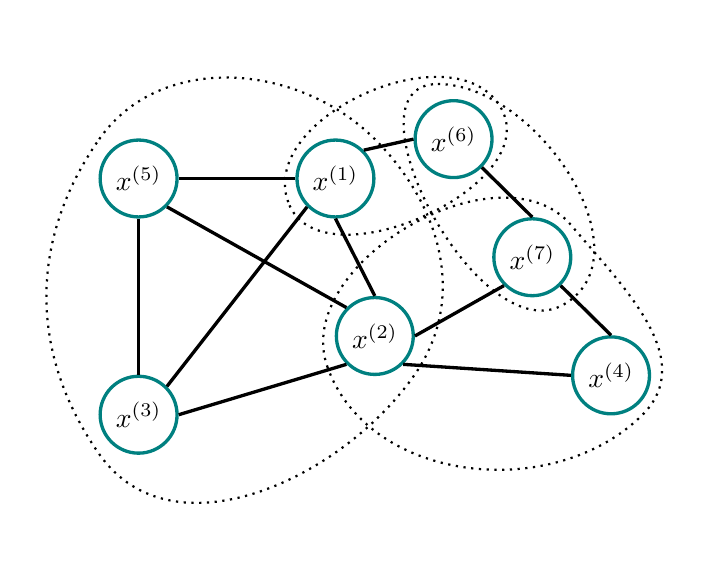
\begin{tikzpicture}[
roundnode/.style={circle, draw=green!50!blue, fill=green!60!blue, very thick, minimum size=7mm},
roundnode2/.style={circle, draw=green!50!blue, very thick, minimum size=9mm},
%squarednode/.style={rectangle, draw=red!60, fill=red!5, very thick, minimum size=5mm},
]
%Nodes
\node[roundnode2] at (2.5,4) (1)     {$x^{(1)}$};
\node[roundnode2] at (3,2) (2)     {$x^{(2)}$};
\node[roundnode2] at (0,1) (3)     {$x^{(3)}$};
\node[roundnode2] at (6,1.5) (4)     {$x^{(4)}$};
\node[roundnode2] at (0,4) (5)     {$x^{(5)}$};
\node[roundnode2] at (4,4.5) (6)     {$x^{(6)}$};
%\node[roundnode] at (1,2.5) (7)     {7};
\node[roundnode2] at (5,3) (8)     {$x^{(7)}$};
%Lines
\draw[-, very thick] (1.west) -- (5.east);
\draw[-, very thick] (1.north east) -- (6.west);
\draw[-, very thick] (1.south) -- (2.north);
%\draw[-, very thick] (1.south west) -- (7.north east);
%\draw[-, very thick] (1.south east) -- (8.west);
\draw[-, very thick] (8.south west) -- (2.east);
\draw[-, very thick] (8.south east) -- (4.north);
\draw[-, very thick] (4.west) -- (2.south east);
\draw[-, very thick] (3.east) -- (2.south west);
%\draw[-, very thick] (3.north east) -- (7.south west);
%\draw[-, very thick] (2.west) -- (7.east);
\draw[-, very thick] (3.north) -- (5.south);
\draw[-, very thick] (6.south east) -- (8.north);
\draw[-, very thick] (5.south east) -- (2.north west);
\draw[-, very thick] (1.south west) -- (3.north east);
%\draw[-, very thick] (5.south east) -- (7.north west);
% \draw[dotted, very thick] (1.north) -- (1a.south);
% \draw[dotted, very thick] (3.north) -- (3a.south);
% \draw[dotted, very thick] (2.north) -- (2a.south);
% \draw[dotted, very thick] (4.north) -- (4a.south);
%Cliques and (-1,0)
%5-1-2-3-5
\draw[dotted, thick] (-0.5,4.5)
    to[out=55,in=135] (3,4.5)
    to[out=315,in=55](3.5,1.5)
    to[out=-125,in=-55] (-0.5,0.5)
    to[out=125,in=-125] (-0.5,4.5);
%6-7-6
\draw[dotted, thick] (3.8,5.2)
    to[out=0,in=30] (5.4,2.4)
    to[out=-150,in=180] (3.8,5.2);
%2-7-4-2
\draw[dotted, thick] (2.4,1.6)
    to[out=110,in=130](5.5,3.4)
    to[out=-50,in=45] (6.4,1)
    to[out=-135,in=-70] (2.4,1.6);
%1-6-1
\draw[dotted, thick] (1.9,3.7)
    to[out=110,in=120](4.6,4.9)
    to[out=-60,in=-70] (1.9,3.7);
\end{tikzpicture}
    \caption[Undirected Random Field of seven nodes including maximum cliques.]{\textbf{Undirected Random Field of seven nodes including maximum cliques.} The random field displayed here can be described with a Graph $\mathcal{G}$. Where $\mathcal{V}$ are all nodes seen in the figure and $\mathcal{E}$ are the edges drawn with a line between nodes. We draw dotted lines around the set of maximum cliques, which are not a full subset of any other clique. Maximum cliques are a set of fully connected nodes with common neighbors. A neighborhood is defined through an edge between two nodes, such as $\{ x^{(1)}, x^{(6)}\} \in \mathcal{E}$. Here $ \{ \{ x^{(1)}, x^{(6)}\}, \{ x^{(1)}, x^{(3)}, x^{(4)}, x^{(5)} \}, \{ x^{(6)}, x^{(7)} \}, \{ x^{(2)}, x^{(4)}, x^{(7)} \} \}$ form the set of maximum cliques.
    On a set of maximum cliques, we can define an energy function, Gibbs distribution or use the \mccorrect{conditional auto regressive model} to define spatial dependencies.
    The precision matrix $\bm{Q}$ represents those spatial dependencies weighted by the hyper parameter $\bm{\theta}$.}
    \label{fig:MRFGRAPH}
\end{figure}

In this subsection, we present the Conditional Auto Regressive (CAR) model and the Gibbs field to define a graph $\mathcal{G}(\mathcal{V},\mathcal{E})$ and the corresponding precision matrix $\bm{Q}$.
For curious readers we recommend the book \cite{bremaud2013markov}.

The CAR method can include neighbouring nodes of numerous orders.
We define the entries of the precision matrix as follows:
\begin{equation}
      Q_{ij} = \begin{cases}
          \kappa_i & i = j \\
        \kappa_i \beta_{ij} & i \neq j
      \end{cases},
  \end{equation}
where $\beta_{ij} = 0 $, if $x^{(i)}$ and $x^{(j)}$ are conditionally independent, and $\kappa_i > 0$ to ensure positive-definiteness of $\bm{Q}$ for all $i = 1, \dots, n$.
The full conditionals are normally distributed
\begin{equation}
    x^{(i)} | x^{(-i)} = x^{(i)} | \partial x^{(i )} \sim \mathcal{N} \big( \underbrace{\sum_{j:j\neq i} \beta_{ij} x^{(j)}}_{\text{mean}}  \, , \, \underbrace{\kappa_i^{-1}}_{\text{variance}} \big)
\end{equation}
and depend only on neighbouring nodes $\partial x^{(i )}$ having an edge to $x^{(i)}$.
We can then write the probability density over all nodes $\bm{x}$ including their means $\bm{\mu}$ as follows:
\begin{align}
    \pi( \bm{x} ) %&= \pi(x_1) \pi(x_2 | x_1) \cdots \pi(x_N | x_{N-1} ) \\
    &= \frac{1}{(2 \pi)^{n/2}} \sqrt{\det(\bm{Q})} \ \, \exp{\Bigg[ - \frac{1}{2} ( \bm{x} - \bm{\mu} )^T \bm{Q} (\bm{x} - \bm{\mu}) \Bigg]} \\ 
     &= \frac{1}{(2 \pi)^{n/2}} |\bm{\Sigma}|^{-1/2} \exp{\Bigg[ - \frac{1}{2} ( \bm{x} - \bm{\mu} )^T \bm{\Sigma}^{-1} ( \bm{x} - \bm{\mu} ) \Bigg]} \, .
\end{align}

Alternatively, we can describe a set of nodes through a Gibbs field, where we define a clique $c \in \mathcal{C}$ as a set of fully connected nodes.
In a clique each node $j \in c$ has mutual neighbours to any other node $i \neq j \in c$. 
If for any node $j \notin c$ and $j \in \mathcal{V}$, the union of $j \cup c$ is not a clique then we call $\tilde{c} \in \mathcal{C}$ a maximal clique.
We conclude that maximal cliques are not a complete subset of another clique.
%\mccorrect{double check if concept of cliques \textbf{and} maximum cliques has to be explained}
The positive clique-potential $\phi_{\tilde{c}}(\tilde{c})$ describes the interactions of all nodes within a clique.
The sum over all maximum clique-potentials is often described as the Energy:
\begin{equation}
    E = \sum_{\tilde{c} \in \mathcal{C}} \phi_{\tilde{c}}(x^{(i)} : x^{(i)} \in c).
\end{equation}
We normalize the Gibbs distribution $\pi(\bm{x})$ of a random field with a normalization constant $Z$.
\begin{align}
    \pi(\bm{x}) &= \frac{1}{Z} \exp{ \Big[ -\sum_{\tilde{c}\in \mathcal{C}} \phi_{\tilde{c}}(x^{(i)} : x^{(i)} \in \tilde{c}) \Big] } \\
    &Z = \sum_{i \in \mathcal{V}} \prod_{\tilde{c} \in \mathcal{C}} \exp{ \Big[ - \phi_{\tilde{c}} (x^{(i)}: x^{(i)} \in \tilde{c}) \Big] } 
\end{align}


The Hammersley-Clifford theorem states that if we describe any Random Field through a Gibbs distribution over maximum cliques then we deal with a MRF.
First proven by Julien Besag we can show that conditional joint distribution is expressed as
\begin{align}
\pi(x^{(i)} | \partial x^{(i)}) &= \frac{1}{Z} \exp{\big[  -\sum_{\tilde{c} \in \mathcal{C}} \phi_{\tilde{c}}(x^{(i)},x^{(j)} : i,j \in \tilde{c} \text{ and } i \neq j) \big]}\\
     &Z = \sum_{i \in \mathcal{V}} \prod_{\tilde{c} \in \mathcal{C}} \exp{ \Big[ - \phi_{\tilde{c}} (x^{(i)},x^{(j)}: i,j \in \tilde{c} \text{ and } i \neq j) \Big] }
\end{align}
and can be found in \cite{besag1974spatial}.
% To actually model an MRF based on a Gibbs field we set up one clique potential and connect the neighbouring sites in a 2D lattice
% \begin{equation}
%     \phi_c(x_i,x_j) = \begin{bmatrix}
%                         x_{i} & x_{j}
%                      \end{bmatrix}  
%                      \underbrace{\begin{bmatrix}
%                         w_{ij} & -w_{ij} \\
%                         -w_{ji} & w_{jj}
%                      \end{bmatrix}}_{\mathbf{W}} 
%                      \begin{bmatrix}
%                         x_{i} \\ x_{j}
%                      \end{bmatrix}  
%                      % \begin{bmatrix}
%                      %    e^{w_{ij}} & e^{-w_{ij}} \\
%                      %    e^{-w_{ji}} & e^{w_{jj}}
%                      % \end{bmatrix} 
% \end{equation}
% if not neighbours the $w_{ij} = 0$, assume symmetrie in within the weight matrix $\mathbf{W}$.
% \begin{align}
%     \ln{ \pi(x_i| \partial x_i) } \propto - \frac{1}{2} \mathbf{x}^T \mathbf{W} \mathbf{x} + \mathbf{b}^T \mathbf{y} \\
%     \pi(x_i| \partial x_i) \propto \exp{\Bigg[- \frac{1}{2} (\mathbf{y} - \mu)^T \mathbf{\Sigma}^{-1} (\mathbf{y} - \mu)  \Bigg]}
% \end{align}
The potential $\phi_{\tilde{c}}$ can describe the interactions between different nodes of a Gaussian Gibbs field if set accordingly, which leads to the precision-matrix $\bm{Q}$ for a Gaussian Markov Random Field (GMRF).
%\mccorrect{For example with specific $\phi_c$/$\bm{Q}$ see application/appendix}





%define nieghbourhood struicture
%\begin{itemize}
  % \item CAR
  
  % % symmetry: $k_i \beta_{ji} = k_j \beta_{ij}$ for all $i \neq j$\\
  % % positive definiteness $\kappa_i > 0$ for all $i = 1, \dots, n$\\
  % % if $Q_{i,j} = 0$ $x_j$ and $x_i$ are conditionally independent\\
  % % if $Q_{i,j} \neq 0$, $\beta_{i,j} \neq 0$ $i \neq j$ then $x_j$ and $x_i $ are conditional dependent, neighbours, have an edge\\
  % % conditional $x_i | x_{-i} = x_i | x_{\partial i } \sim \mathcal{N}(\underbrace{\sum_{j:j\neq i} \beta_{i,j} x_j}_{\text{mean}}  \, , \, \underbrace{\kappa_i^{-1}}_{\text{variance}} )$\\
  % % choose $\beta and \kappa $
  
  % \item cliques

  
  %\item specify Q directly
  % \item Gibbs Distribution

  %  The Markov property describes conditional dependence of image signals within a local neighbourhood system, which is proved to be useful in capturing and modelling usually highly localised and coherent texture features. Another appealing property of an MRF is that, by the Hammersley-Clifford theorem [42], an MRF can be characterised by a global Gibbs distribution. \\
  %  define cliques\\
  %  define maximum cliques\\
  %  maximum clique potential\\
  %  \begin{equation}
  %      E() = \sum_{c_i \in \mathcal{C}} \Phi(x_j : j \in c_i)
  %  \end{equation}
  %  \begin{equation}
  %      Pr() = \frac{1}{Z} \exp{ \{  - E  \} }
  %  \end{equation}
  %  normalisation\\
  %  \begin{equation}
  %      \pi(x_i | \partial x_i) = \frac{1}{Z_i} \exp{}
  %  \end{equation}
   
  %  Hammersley-Clifford Theorem, besag\\
  %  MRF condintional \\
  %  choose function $\phi$
   
%\end{itemize}

\section{linear-Gaussian hierarchical Bayesian model}
\label{sec:Bayesian}
Bayesian hierarchical models are a very helpful tool to describe a measurement process through different layers of complexity.
It allows us to backtrack from our observations to the source of the measurement in a \mccorrect{very precise/simplified} way.
Here we closely follow the terminology of \cite{fox2016fast, simpson2012think}


\begin{figure}[thb!]
    \centering
    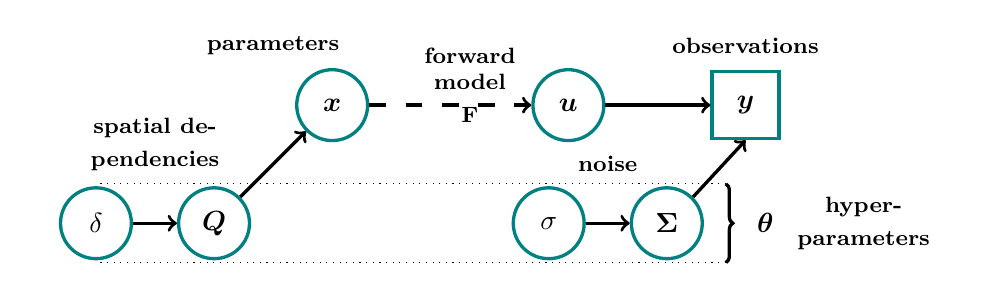
\begin{tikzpicture}[
roundnode/.style={circle, draw=green!50!blue, fill=green!60!blue, very thick, minimum size=7mm},
roundnode2/.style={circle, draw=green!50!blue, very thick, minimum size=9mm},
rectnode/.style={rectangle, draw=green!50!blue, very thick, minimum size=8.5mm},
mydotted/.style = {dash pattern=on 6.1pt off 7pt},
%squarednode/.style={rectangle, draw=red!60, fill=red!5, very thick, minimum size=5mm},
]
%Nodes
%\node[roundnode] at (0,0) (1)     {1};
\node[roundnode2] at (-1.5,-1.5) (H1)     {$\bm{Q}$};
\node[roundnode2] at (0,0) (1)     {$\bm{x}$};
\node[roundnode2] at (3,0) (2)    {$\bm{u}$};
\node[rectnode] at (5.25,0) (3)    {$\bm{y}$};
\node[roundnode2] at (4.25,-1.5) (H3)    {$\bm{\Sigma}$};
\node[roundnode2] at (2.75,-1.5) (HN)    {$\sigma$};
\node[roundnode2] at (-3,-1.5) (HP)    {$\delta$};
%text
\draw (1.75,0.25) node[align=center, text width=1.5cm] {\footnotesize \textbf{forward model \\ F}};
\draw (6.75,-1.5) node[align=center, text width=2.5cm] {\footnotesize \textbf{hyper\-parameters}};
\draw (5.5,-1.5) node[align=center, text width=0.5cm] { $\bm{\theta}$};
\draw (5.25,0.75) node[align=center, text width=3cm] {\footnotesize \textbf{observations}};
\draw (-0.75,0.75) node[align=center, text width=3cm] {\footnotesize \textbf{parameters}};
\draw (-2.25,-0.5) node[align=center, text width=3cm] {\footnotesize \textbf{spatial dependencies}};
%\draw (-1.4,-2.3) node[align=center, text width=3cm] {\footnotesize \textbf{hyper-prior}};
\draw (3.5,-0.75) node[align=center, text width=3cm] {\footnotesize \textbf{noise}};
% Calligraphic brace
\draw[very thick, decorate,decoration = {brace}] (5,-1) --  (5,-2);

%Lines
\draw[->, very thick] (HN.east) -- (H3.west);
\draw[->, very thick] (HP.east) -- (H1.west);
\draw[->, very thick] (H1.north east) -- (1.south west);
\draw[->, mydotted, very thick] (1.east) -- (2.west);
\draw[->, very thick] (2.east) -- (3.west);
\draw[->, very thick] (H3.north east) -- (3.south);
\draw[dotted] (5,-1) -- (-3,-1);
\draw[dotted] (5,-2) -- (-3,-2);
\end{tikzpicture}
    \caption[A hierarchical Bayesian model describes how we model a physical process to observe data.]{\textbf{A Bayesian hierarchical model describes how we model a physical process to observe data.} Through a forward model we describe a physical process depending on some parameters $\bm{x}$.
    The spatial dependencies of those parameters $\bm{x}$ are described through the hyper-parameters $\bm{\theta} = (\delta, \sigma)$.
    The precision matrix $\bm{Q}$ is defined according to our \changelinkcolor{black}\hyperref[subsec:MRF]{Markov Random field} and the amount of interaction between certain nodes is described by $\delta$.
    The forward map $\bm{F}$ models a physical process and maps the parameters $\bm{x}$ to a space of all measurable $\bm{u}$.
    From this space $\bm{u}$, we observe some data including some random noise $\gamma$ with variance $\bm{\Sigma}(\gamma)$.
    A Bayesian framework allows us to find the most likely parameters and hyper-parameters $\bm{x}, \bm{\theta}| \bm{y}$ given our measurement .}
    \label{fig:BAYHIER}
\end{figure}

Usually, a measurement device delivers some data $\bm{y}$ including some noise $\sigma$ and we like to model the observation to quantify some unknown parameters $\bm{x}$ and their unknown spatial dependencies.
%Given the observed data vector $\bm{y}$ we would like to quantify the unknown parameter vector $\bm{x}$, including the uncertainty of $\bm{x}$, and the hyper-parameter vector $\bm{\theta}$. corresponding to the hyper-prior $\pi ( \bm{\theta} ) $ 
%As discussed in the subsection, we set up a graphical model to describe spatial dependencies within our parameter field, as seen in figure \ref{fig:MRFGRAPH} $\bm{x|\bm{\theta}}$.
Through the precision matrix $\bm{Q}(\delta)$, we define neighborhoods and weight pair-wise interactions of parameters $x^{(j)} \text{ and } x^{(i)}$ according to a hyper-prior distribution $\pi ( \delta ) $ in (\ref{eq:hyper}).
The inverse of the precision matrix $\bm{Q}( \delta ) $ is the variance of the prior distribution $\pi(\bm{x} |  \bm{Q}^{-1}( \delta ) )$ in (\ref{eq:prior}), and usually sparse.
Based on this graphical model we map $\bm{x}$ through a forward model $\bm{F}$ \mccorrect{Dimensions} to space of all measurables $\bm{u}$.
%Given a forward model $\bm{F}$, which typically describes a physical process, we map the parameters to a so-called space of all measurable $\bm{u}$.
Next, we observe some data $\bm{y} = \bm{F} \bm{x} + \gamma$ and add some unknown normally distributed random noise $\eta$ with variance $\bm{\Sigma}(\gamma)$.
We assume that this noise vector is independent and identically distributed (i.i.d.).
The likelihood function $\pi( \bm{y} | \bm{x, \theta} )$ in (\ref{eq:likeli}) describes how likely/realistic the observations $\bm{y}$ are.
In our specific case, we choose a linear forward model and a Gaussian prior, so that our likelihood function and posterior distribution in (\ref{eq:post}) are normally distributed as well.
In doing so we can find an analytic expression for the uncertainty of the posterior and see that it is depending on both the prior and the likelihood distribution, for more details we refer to the Appendix \ref{ap:bayesian}.

In Equations (\ref{eq:prior}) - (\ref{eq:hyper}), we summarize a hierarchical Bayesian model in a generalized form, with the hyper-parameter $\bm{\theta} = (\delta, \gamma)$.
Note that in this case we define two hyper-parameters, but we can increase the dimensions of $\theta$ to an arbitrary number suitable to describe the underlying physical process sufficiently.
\begin{subequations}
\begin{align}
     \label{eq:likeli}
    \bm{y|x, \theta} &\sim \mathcal{N}(\bm{F x}, \bm{\Sigma}(\bm{\theta}) ) \qquad \quad   \, \text{(likelihood)}\\
    \label{eq:prior}
    \bm{x| \theta} &\sim \mathcal{N}(\bm{\mu}, \bm{Q}^{-1}(\bm{\theta}) ) \qquad \qquad  \quad \! \! \! \text{(prior)} \\
    \label{eq:hyper}
    \bm{\theta} &\sim \pi(\bm{\theta}) \qquad \qquad \qquad \qquad \quad \; \, \text{(hyper-prior)}
 \end{align}
 The posterior has the following from
 \begin{align}
     \label{eq:post}
    \bm{x , \theta|y} &\sim \mathcal{N}( \mu_{\bm{x , \theta|y} } , ( \bm{Q} + \bm{F}^T\bm{\Sigma}^{-1}\bm{F} )^{-1} ) \quad  \text{(posterior)}
\end{align}
\end{subequations}
with the mean $\mu_{\bm{x , \theta|y} } = \bm{\mu} + (\bm{Q} + \bm{F}^T \bm{\Sigma}^{-1} \bm{F})^{-1} \bm{F}^T \, \bm{\Sigma}^{-1} (\bm{y} - \bm{F \mu})$. 


Using \mccorrect{Bayes} theorem we can find an expression for the posterior distribution $\pi (\bm{x} , \bm{\theta} | \bm{y})$ for the parameters $\bm{x}$ and the hyper-parameters $\bm{\theta}$ given the observed data $\bm{y}$.
\begin{align}
    \pi (\bm{x} , \bm{\theta} | \bm{y}) &= \frac{\pi( \bm{y} | \bm{x}, \bm{\theta} ) \, \pi(\bm{x},  \bm{\theta}) }{\pi(\bm{y})}
    %& \propto \pi( \bm{y} | \bm{x}, \bm{\theta} ) \, \pi(\bm{x} |  \bm{\theta}) \pi( \bm{\theta} )
\end{align}

%We obtain a posterior probability distribution proportional to the distribution in our Bayesian hierarchical model, see equations \ref{eq:hyper} - \ref{eq:likeli}.
If we like to compute the posterior distribution we have to compute the normalization constant $\pi(\bm{y})$, where we marginalize out $\bm{x}$ and $\bm{\theta}$ :
\begin{equation}
    \pi(\bm{y}) = \int \int \pi(\bm{y}, \bm{x}, \bm{\theta}) \diff \bm{x} \diff \bm{\theta} \, ,
\end{equation}
which can yield a extensive computation.
% Usually this is computationally too expensive, but if we assume that the normalization constant $\pi(\bm{y}) $ is finite and non zero
% we obtain a posterior proportional to the distribution in our hierarchical model:
% \begin{align}
%     \pi (\bm{x} , \bm{\theta} | \bm{y}) \propto \pi( \bm{y} | \bm{x}, \bm{\theta} ) \, \pi(\bm{x} |  \bm{\theta}) \pi( \bm{\theta} ) \, .
% \end{align}
Using the posterior density we can find the expected value of any function $h(\bm{x})$ though an average of the function weighted by the probability density distribution $\pi (\bm{x} , \bm{\theta} | \bm{y})$.
\begin{equation}
    \text{E}_{\bm{x},\bm{\theta}|\bm{y}} [h(\bm{x})] = \int \int h(\bm{x}) \pi( \bm{x}, \bm{\theta} | \bm{y}) \diff \bm{x} \diff \bm{\theta} 
\end{equation}

\mccorrect{Taking a look at the posterior we can see that $\pi(\bm{x}, \bm{\theta} | \bm{y})$.. and see that to solve this might be very tidious, where as the ratio is much easier...}
\begin{align}
    \pi(\bm{x}, \bm{\theta} | \bm{y}) &\propto  \pi(\bm{y}|  \bm{x}, \bm{\theta} )  \pi(\bm{x}|  \bm{\theta} )  \pi(\bm{\theta} ) \\
    &= \frac{  \pi(\bm{\theta})}{\sqrt{ \det( \bm{\Sigma}) \,  \det( \bm{Q} )^{-1}  } } \exp{ \Bigg[  \frac{(\bm{F \mu} - \bm{y})^T  (\bm{F \mu} - \bm{y})}{\bm{\Sigma}} + \frac{(\bm{\mu} - \bm{x})^T  (\bm{\mu} - \bm{x}) }{\bm{Q}^{-1}}\Bigg] }
\end{align}

If we set $h(\bm{x}) = \bm{x}$ we get the mean of the parameter $\bm{x}$ or the posterior covariance if $h(\bm{x}) = (\bm{x} - \text{E}_{\bm{x},\bm{\theta}|\bm{y}} [\bm{x}]) (\bm{x} - \text{E}_{\bm{x},\bm{\theta}|\bm{y}} [\bm{x}] )^T $.
Computing that is very expensive and usually not feasible as the parameters can too many different values, depending on the range and complexity of the problem.
Instead, we can explore the parameter space for a few (e.g. $10^4$) discrete values and use the Monte-Carlo method to approximate the integral.
%and compare in between the generated samples of the posterior.
%One way of moving and picking values in our parameter space is through a so-called Markov-chain Monte Carlo (MCMC) algorithm.


\subsection{Monte-Carlo Method Integration}
The Monte-Carlo method was first developed in Los Alamos, United States of America, just after the II world war to simulate the flight path of neutrons.
Later in 1949, N. Metropolis and S. Ulam formulated their ideas already suggesting to use 'Markoff' chains in Monte Carlo simulations to approximate continuous functions \cite{metropolis1949monte}.
%Using random values .
For more details on the fundamental theorems we use in this work, we refer to the books \cite{hammersley1964general, whitlock1986monte}

Using the Monte-Carlo method we can approximate the expected value of any function $h(\bm{x})$ by the sample mean:
\begin{equation}
\label{eq:sampMean}
    \text{E}_{\bm{x},\bm{\theta}|\bm{y}} [h(\bm{x})] =  \int \int   \bm{x} \,  \pi(\bm{x}, \bm{\theta} | \bm{y} ) \, \text{d} \bm{x}  \, \text{d} \bm{\theta} \approx \frac{1}{N +1} \sum_{i=0}^{N} \bm{x}_{i} \, ,
\end{equation}
where we draw $n$ parameter samples $\bm{x}_{i}$ from the posterior distribution $\pi (\bm{x} , \bm{\theta} | \bm{y})$.
%If we set $h(\bm{x}) = \bm{x}$ we get the mean or the posterior covariance if $h(\bm{x}) = (\bm{x} - \text{E}_{\bm{x},\bm{\theta}|\bm{y}} [\bm{x}]) (\bm{x} - \text{E}_{\bm{x},\bm{\theta}|\bm{y}} [\bm{x}] )^T $.
We can argue with the central limit theorem that if $N \rightarrow \infty$ the sequence of $ \{ \bm{x}_{0}, \dots, \bm{x}_{N} \}$ converges the sample mean and sample variance to the true mean and true covariance of $\pi( \bm{x}, \bm{\theta} | \bm{y})$.
In our case, we know that the posterior is normally distributed and the task now is to draw samples from this distribution to perform such an integration.
The problem is that it is not feasible to compute the posterior distribution due to the size of the parameter space.
Instead, we construct a Markov chain of randomly picked parameters, which converges to the posterior distribution.

\subsection{Markov Chains}
\label{subsec:Markov}
First formulated by Andrey Markov and published in 1906, Markov chains are a very useful statistical tool to describe real-world processes \cite{markov2006extension}. 
In this section, we discuss some of the properties of Markov chains to make sure that we sample from a unique equilibrium distribution, which is in our case the posterior distribution $\pi (\bm{x} , \bm{\theta} | \bm{y})$.
We like to show aperiodicity, irreducibility, and convergence towards a stationary distribution by proofing the detailed balance condition.
If all of these properties hold we call a chain ergodic with a unique equilibrium distribution, e. g. $\pi (\bm{x} , \bm{\theta} | \bm{y})$.
For more detailed information we refer to \cite{fox2010introduction, bremaud2013markov}.

%\mccorrect{ergodic chain convergence guaranteed by the central limit theorem}
%We explore the parameter space of our Bayesian hierarchical model and generate a Markov chain.
%For the sequence of parameter values we calculate the corresponding posterior distribution.
%We require this Markov chain to be ergodic.
%This means that the chain converges to an equilibrium distribution, which is in our case the posterior distribution, and each drawn state is reachable by any other state, meaning the chain is aperiodic.

%Markov
In a finite parameter space $\Omega(\mathcal{X},\mathcal{\theta})$ we draw a sequence of random variables  $ \mathcal{M} = \big \{ \{ \bm{x}_0, \bm{\theta}_0 \} , \{ \bm{x}_1, \bm{\theta}_1 \} , \dots , \{ \bm{x}_N, \bm{\theta}_N \} \big \}$ from distributions $ \pi^{(0)}, \dots , \pi^{(N)}$  .
The Markov condition requires that each transition probability $\text{Pr}(\cdot)$ of a new state $\{ \bm{x}_{N+1}, \bm{\theta}_{N+1} \}$ only depends on the current state $\{ \bm{x}_{N}, \bm{\theta}_{N}\}$:
\begin{align}
    \text{Pr}(\{ \bm{x}_0, \bm{\theta}_0 \} , \{ \bm{x}_1, \bm{\theta}_1 \} , \dots , \{ \bm{x}_N, \bm{\theta}_N \}) &=  \text{Pr}(\{ \bm{x}_{N+1}, \bm{\theta}_{N+1} \}| \{ \bm{x}_N, \bm{\theta}_N \} \, .
\end{align}

%distributions
For reasons of simplicity in terminology we denote the state $\{ \bm{x}_N, \bm{\theta}_N \}$ as vector $(\bm{x}^T_N, \bm{\theta}^T_N )^T = \bm{i}$
The probability for the Markov chain to be in that state $\bm{i}$ after $N$ steps is denoted as $\pi^{(N)}_{\bm{i}} = \text{Pr}( (\bm{x}^T_N, \bm{\theta}^T_N )^T = \bm{i})$.
We arrange the probability distribution of the $N$th step as a row vector representing the probabilities to be in different states $\bm{i},\bm{j} \in \Omega( \mathcal{X}, \mathcal{\theta} )$
\begin{align}
     \pi^{(N)} = \begin{bmatrix}
          \cdots 
           \pi^{(N)}_{\bm{i}} 
          \pi^{(N)}_{\bm{j}} 
          \cdots 
         \end{bmatrix}
\end{align}


%homogenous
A Markov chain $\mathcal{M}$ is homogeneous if the transition probability only depends on the value of the current and proposed state and not on $n$, the position in the chain.
\begin{equation}
    \text{Pr}(\{ \bm{x}_{N+M+1}, \bm{\theta}_{N+M+1} \}| \{ \bm{x}_{N+M}, \bm{\theta}_{N+M} \}) = \text{Pr}(\{ \bm{x}_{N+1}, \bm{\theta}_{N+1} \}| \{ \bm{x}_N, \bm{\theta}_n \} ) \quad \forall M \in \mathbb{Z}
\end{equation}
Then we denote the probability to transition from state $\{ \bm{x}_N, \bm{\theta}_N \} = i$ to $\{ \bm{x}_{N+1}, \bm{\theta}_{N+1} \}= j $ as an element of the transition matrix $\bm{P}$:
\begin{equation}
    P_{\bm{i j}} =  \text{Pr}( ( \bm{x}^T_{N+1}, \bm{\theta}^T_{N+1} )^T = \bm{j}| ( \bm{x}^T_N, \bm{\theta}^T_N )^T  = \bm{i}) 
\end{equation}
This matrix represents the transitions for one step from
%stationary distribution
As we draw more and more states, some of those states are more likely to occur than others.
The Chain will reach an equilibrium distribution $\pi^{(N)} \rightarrow \pi$ as $N \rightarrow \infty$.
We call $\pi$ the stationary distribution for the transition matrix $\bm{P}$.
Here, $\pi$ is the left eigenvector of $\bm{P}$ with the eigenvalue one such that
\begin{equation}
    \pi = \pi \bm{P} \, .
\end{equation}
Once we draw values of that chain from the stationary distribution, the distribution does not change.


%define and explain
%irreducable
A Markov chain is irreducible if all states in $\Omega$ intercommunicate.
That means for any two states  $( \bm{x}_N^T, \bm{\theta}_N^T )^T = \bm{i}$ and $( \bm{x}^T_{N+1}, \bm{\theta}^T_{N+1} )^T= \bm{j} $ we can find a path with non-zero probability linking $\bm{i} \rightarrow \bm{j}$ and a path linking  $\bm{i} \leftarrow \bm{j}$.
Then the state space $\Omega$ is irreducible under $\bm{P}$.
Within an irreducible chain, all states have the same period.

%aperiodic
A period is the number of steps for a chain to revisit a set of states starting from the same set of states.
An aperiodic chain has period one.
If we are allowed to stay in a state $i$, so that the self-transition  $P_{\bm{i,i}} > 0$, we can break any periodic pattern and the chain is aperiodic.

%ergodic
If a Markov chain is aperiodic and irreducible then this chain is ergodic.
For an ergodic Markov chain on a finite state space $\Omega$, there exists a stationary distribution $\pi$.
This stationary distribution is unique if it satisfies the detailed balance condition.
\begin{align}
    \pi(\{ \bm{x}_{N+1}, \bm{\theta}_{N+1} \} = \bm{j} ) P_{\bm{j,i}} &= \pi(\{ \bm{x}_N, \bm{\theta}_N \} = \bm{i}) P_{\bm{i,j}}\\
    \pi_{\bm{j}}  P_{\bm{j,i}} &= \pi_{\bm{i}} P_{\bm{i,j}}
\end{align}

In a large class of Markov chains the detailed balance condition is very helpful to find the stationary distribution.


%consequences of the ergodic theorem
As a consequence of the ergodic theorem, we observe an unique equilibrium distribution $\pi^{(N)} \rightarrow \pi$ as $N \rightarrow \infty$ independent of the initial distribution  $\pi^{(0)}$.
Now, we sample from the posterior distribution and can calculate the sample mean, as seen in Equation (\ref{eq:sampMean}).

Next, we like to generate such a chain and define the transition probabilities using the Metropolis-Hastings algorithm.
%The Metropolis-Hastings algorithm is a Markov chain Monte Carlo algorithm and fulfills all of the stated properties for Markov Chains so it generates a chain that converges towards the desired posterior distribution.

%+++++++++++++++++++++++++++++++++++++++++++++++++++ extra Markov Chapter ++++++++

% \subsection{Markov-Chains}
% \label{subsec:Markov}
% In this section, we discuss some of the properties of Markov chains to make sure that we sample from a unique equilibrium distribution, which is in our case the posterior distribution $\pi (\bm{x} , \bm{\theta} | \bm{y})$.
% We like to show aperiodicity, irreducibility, and convergence towards a stationary distribution by proofing the detailed balance condition.
% If all of these properties hold we call a chain ergodic with a unique equilibrium distribution.
% For reasons of simplicity and illustration purposes, we consider one-dimensional chains in this subsection, for information we refer to \cite{fox2010introduction, bremaud2013markov}.
% %\mccorrect{ergodic chain convergence guaranteed by the central limit theorem}
% %We explore the parameter space of our Bayesian hierarchical model and generate a Markov chain.
% %For the sequence of parameter values we calculate the corresponding posterior distribution.
% %We require this Markov chain to be ergodic.
% %This means that the chain converges to an equilibrium distribution, which is in our case the posterior distribution, and each drawn state is reachable by any other state, meaning the chain is aperiodic.

% %Markov
% In a finite state space $\Omega(\mathcal{X} )$ we draw a finite sequence of correlated random variables  $ \mathcal{M} = \{ x_0, x_1 , \dots ,  x_n   \}$ from distributions $ \pi^{(0)}, \dots , \pi^{(n)}$  .
% The Markov condition requires that each transition probability $\text{Pr}(\cdot)$ of a new state $x_{n+1}$ only depends on the current state $ x_n $:
% \begin{align}
%    \text{Pr}( x_{n+1}| x_{n}) &= \text{Pr}(x_{n+1}| x_{n}, x_{n-1}, \dots , x_{0})  \, .
% \end{align}

% %distributions
% The probability for the Markov chain to be in $x_n = i$ after $n$ steps is denoted as $\pi^{(n)}_i = \text{Pr}( x_n = i)$.
% We arrange the probability distribution of the $n$th step as a row vector representing the probabilities to be in different states $i,j \in \Omega( \mathcal{X} )$
% \begin{align}
%      \pi^{(n)} = \begin{bmatrix}
%           \cdots 
%            \pi^{(n)}_{i} 
%           \pi^{(n)}_{j} 
%           \cdots 
%          \end{bmatrix}
% \end{align}


% %homogenous
% A Markov chain $\mathcal{M}$ is homogeneous if the transition probability only depends on the value of the current and proposed state and not on $n$, the position in the chain.
% \begin{equation}
%     \text{Pr}(x_{n+m+1}| x_{n+m}) = \text{Pr}( x_{n+1}| x_{n}) \quad \forall m \in \mathbb{Z}
% \end{equation}
% Then we denote the probability to transition from state $ x_{n} = i$ to $ x_{n+1}= j $ as an element of the stochastic transition matrix $\bm{P}$:
% \begin{equation}
%     P_{i j} =  \text{Pr}( x_{n+1} = j| x_{n}  = i) 
% \end{equation}
% %stationary distribution
% As we draw more and more states, some of those states are more likely to occur than others.
% The Chain will reach an equilibrium distribution $\pi^{(n)} \rightarrow \pi$ as $n \rightarrow \infty$.
% We call $\pi$ the stationary distribution for the transition matrix $\bm{P}$.
% Here, $\pi$ is the left eigenvector of $\bm{P}$ with the eigenvalue one such that
% \begin{equation}
%     \pi = \pi \bm{P} \, .
% \end{equation}
% Once we draw values of that chain from the stationary distribution, the distribution does not change.


% %define and explain
% %irreducable
% A Markov chain is irreducible if all states in $\Omega$ intercommunicate.
% That means for any two states  $ x_{n} = i$ and $ x_{n+1}= j $ we can find a path with non-zero probability linking $i \rightarrow j$ and a path linking  $i \leftarrow j$.
% Then the state space $\Omega$ is irreducible under $\bm{P}$.
% Within an irreducible chain, all states have the same period.

% %aperiodic
% A period is the number of steps for a chain to revisit a set of states starting from the same set of states.
% An aperiodic chain has period one.
% If we are allowed to stay in a state $i$, so that the self-transition  $P_{ii} > 0$, we can break any periodic pattern and the chain is aperiodic.

% %ergodic
% If a Markov chain is aperiodic and irreducible then this chain is ergodic.
% For an ergodic Markov chain on a finite state space $\Omega$, there exists a stationary distribution $\pi $.
% This stationary distribution is unique if it satisfies the detailed balance condition.
% \begin{align}
%     \pi( x_{n+1}= j ) P_{ji} &= \pi( x_{n} = i) P_{ij}\\
%     \pi_j  P_{ji} &= \pi_i P_{ij}
% \end{align}
% In a large class of Markov chains the detailed balance condition is very helpful to find the stationary distribution.


% %consequences of the ergodic theorem
% As a consequence of the ergodic theorem, we observe an equilibrium distributing $\pi^{(n)} \rightarrow \pi$ as $n \rightarrow \infty$ independent of the initial distribution  $\pi^{(0)}$.
% Now, we sample from the posterior distribution and can calculate the sample mean, as seen in equation.%\ref{}.

% Next, we like to generate such a chain and define the transition probabilities using the Metropolis-Hastings algorithm.
% The Metropolis-Hastings algorithm is a Markov chain Monte Carlo algorithm and fulfills all of the stated properties for Markov Chains so it generates a chain that converges towards the desired posterior distribution.


%+++++++++++++++++++++++++++++++++++++++++++++++++++++++++++++++++++++++++++++++++ extra Markov chapter




% The probability to be in the state $ \{ \bm{x}, \bm{\theta} \}^{(t)}$ is $\pi^{(t)} = \pi(\{ \bm{x}, \bm{\theta} \}^{(t)}) = \text{Pr}( \{ \bm{x}, \bm{\theta} \}^{(t)}) $.
% We write this as the magrinalization over the whole parmeter space for the previous state and use Bayes theorem to show \mccorrect{...}.
% \begin{align}
%     \text{Pr}( \{ \bm{x}, \bm{\theta} \}^{(t+1)}) &=  \sum_{\{ \bm{x}, \bm{\theta} \}^{(t)} \in \Omega} \text{Pr}( \{ \bm{x}, \bm{\theta} \}^{(t+1)}, \{ \bm{x}, \bm{\theta} \}^{(1)})\\
%     &= \sum_{\{ \bm{x}, \bm{\theta} \}^{(t)} \in \Omega} \text{Pr}(\{ \bm{x}, \bm{\theta} \}^{(t+1)}| \{ \bm{x}, \bm{\theta} \}^{(t)}) \text{Pr}( \{ \bm{x}, \bm{\theta} \}^{(0)}) \\ 
%     \Rightarrow \pi^{(t+1)} &= \sum_{\{ \bm{x}, \bm{\theta} \}^{(t+1)} \in \Omega}  \pi^{(t)}  P_{t,t+1}  = \pi^{(t)} \bm{P} 
% \end{align}
% For $ t \rightarrow \infty$  we have a equilibrium distributing $ \pi $
% \begin{equation}
%     \pi^{(t+1)} = \bm{P} \pi^{(t)}  \xrightarrow{t \rightarrow \infty} \pi = \bm{P} \pi 
% \end{equation}
% This mean very sample i take is from the same distribtion and my chain converges, which i can also proof with the central limit theorem.
% We call this an erigodic Markov chain where we each state can reach any othet state so that $P_{t,t+1} > 0 :  \forall t $, which implies that the Markov chain aperiodic.
% We use a Metroplis Hastings algorithm to construct such a Markov chain.
% \clearpage



% After t steps we have the probability distribution $\text{Pr}( \{ \bm{x}, \bm{\theta} \}^{(p)})$, which reaches state $ \{ \bm{x}, \bm{\theta} \}^{(p)}$.
% If we set then number of steps to $t=1$ and sum over all possible state space/marginalize
% \begin{align}
%     \text{Pr}( \{ \bm{x}, \bm{\theta} \}^{(1)}) &=  \sum_{\{ \bm{x}, \bm{\theta} \}^{(0)} \in \Omega} \text{Pr}( \{ \bm{x}, \bm{\theta} \}^{(1)}, \{ \bm{x}, \bm{\theta} \}^{(0)})\\
%     &= \sum_{\{ \bm{x}, \bm{\theta} \}^{(0)} \in \Omega} P_{0,1} \text{Pr}( \{ \bm{x}, \bm{\theta} \}^{(0)})
% \end{align}


% If we sample froma stationary distribtuion the transition matrix is invariant to the distribution
% \begin{equation}
%     \text{Pr}(\{ \bm{x}, \bm{\theta} \}^{(p+1)}, \{ \bm{x}, \bm{\theta} \}^{(p)}) = \text{Pr}(\{ \bm{x}, \bm{\theta} \}^{(p+1)}| \{ \bm{x}, \bm{\theta} \}^{(p)}) \text{Pr}( \{ \bm{x}, \bm{\theta} \}^{(p)})
% \end{equation}
% then we call this sequence a markov chain.
% It ergodic if it irreducible and aperiodic.


% We deal with an erdogic chain if we have a unique stationary distribution
% which means that we converge to the distributin as t goes to infinty and

% irreducable and aperiodic


% We denote a n
% The Markov chain is ergoic , that means that it is possible to get from every state to every other one
% and sample from an stationary distribution

% As we would like to explore the parameter space and test different states of those parameters we can describe this process through a Markov chain.
% Suppose we have a sequence of $t$ correlated states $ \{ \bm{x}, \bm{\theta} \}^{(0)} , \{ \bm{x}, \bm{\theta} \}^{(1)} , \dots , \{ \bm{x}, \bm{\theta} \}^{(p)} \sim   \pi (\bm{x} , \bm{\theta} | \bm{y}) $, which are drawn from the posterior probability distribution of our previously defined Bayesian model.
% For this chain the Markov Condition holds, so that each state only depends on the previous state.
% \begin{align}
%     \text{Pr}(\{ \bm{x}, \bm{\theta} \}^{(p+1)}| \{ \bm{x}, \bm{\theta}\}^{(p)}, \{ \bm{x}, \bm{\theta} \}^{(p-1)}, \dots , \{ \bm{x}, \bm{\theta}\}^{(0)}) &=  \text{Pr}(\{ \bm{x}, \bm{\theta} \}^{(p+1)}| \{ \bm{x}, \bm{\theta} \}^{(p)})
% \end{align}
% We denote a new proposed state as $  \{ \bm{x}, \bm{\theta} \}^{(p+1)} = \{ \bm{x}, \bm{\theta} \}' $ and state that a Markov chain is also reversible:
% \begin{align}
%     \text{Pr}(\{ \bm{x}, \bm{\theta} \}| \{ \bm{x}, \bm{\theta}\}') &=  \text{Pr}(\{ \bm{x}, \bm{\theta} \}'| \{ \bm{x}, \bm{\theta} \}) \\
%     \Leftrightarrow \text{Pr}(\{ \bm{x}, \bm{\theta} \}| \{ \bm{x}, \bm{\theta} \}') \pi(\bm{x}, \bm{\theta} | \bm{y}) &=  \text{Pr}(\{ \bm{x}, \bm{\theta} \}'| \{ \bm{x}, \bm{\theta} \}) \pi(\bm{x}', \bm{\theta}' | \bm{y}') \\
%     \Leftrightarrow \text{Pr}(\{ \bm{x}, \bm{\theta} \}| \{ \bm{x}', \bm{\theta}'\}) \pi( \bm{y} | \bm{x}, \bm{\theta} ) \, \pi(\bm{x} ,  \bm{\theta}) &=  \text{Pr}(\{ \bm{x}', \bm{\theta}' \}| \{ \bm{x}, \bm{\theta} \}) \pi( \bm{y}' | \bm{x}', \bm{\theta}' ) \, \pi(\bm{x}' , \bm{\theta}') 
% \end{align}
% $\text{Pr}(\{ \bm{x}, \bm{\theta} \}'| \{ \bm{x}, \bm{\theta}\}) $ is the transition probability for a new state $\{ \bm{x}, \bm{\theta} \}'$ given $\{ \bm{x}, \bm{\theta} \}$.
% If we accept those states we use MCMC.

\section{Sampling from the posterior distribution}
In this Section we present the major sampling algorithms which allow us to generate a Markov chain of posterior samples and to characterize the posterior distribution.
\mccorrect{We introduce the Metroplis-Hastings, Gibbs, MTC sampler, T-walk, adaptive MCMC.}


\subsection{Metropolis-Hastings - Markov chain Monte-Carlo}
\label{subsec:MetroHast}
%\cite{hastings1970monte}
%\mccorrect{Why ? one of the most common ones or based for further ....}
Here we introduce the Metropolis-Hastings algorithm, which is a Markov-chain Monte Carlo (MCMC) algorithm.
First published in 1970 and based on the work of Metropolis et. al in 1953 this algorithm provides a framework to find samples from the posterior efficiently \cite{hastings1970monte, metropolis1953equation}.
Generating a Markov-Chain $\{ \bm{x}_0, \bm{\theta}_0 \}, \dots, \{ \bm{x}_j, \bm{\theta}_j \}, \dots, \{ \bm{x}_N, \bm{\theta}_N \}$ we accept and reject proposed samples to accurately calculate the sample mean.



\begin{algorithm}[!thb]
    \caption{Metropolis-Hastings step to  generate a new candidate in a Markov chain}
    \label{alg:metroHasti}
    \SetAlgoLined
    \nonl \textbf{Let}  $\{ \bm{x}_j, \bm{\theta}_j \}$ be the current state , then we \textbf{generate} $\{ \bm{x}_{j+1}, \bm{\theta}_{j+1} \}$ as follows: \\
    \textbf{Draw}: new state $\{ \bm{x}', \bm{\theta}' \}  \sim  g(\bm{x}', \bm{\theta}'|\bm{x}_j, \bm{\theta}_j )$  \\
    \textbf{Acceptance probability}: $\alpha(j+1|j) \equiv \min 
    \begin{rcases}
        \begin{dcases}
            1, \frac{\pi( \bm{x}', \bm{\theta}' | \bm{y}) g(\bm{x}_j, \bm{\theta}_j|\bm{x}', \bm{\theta}' )}{\pi( \bm{x}_{j+1}, \bm{\theta}_{j+1}| \bm{y}) g(\bm{x}', \bm{\theta}'|\bm{x}_j, \bm{\theta}_j )}
        \end{dcases}
    \end{rcases} $ \\
    \textbf{Draw}: $ u \sim \mathcal{U}(0,1)$ \\ 
    {\If{$u \leq \alpha(j+1|j)$}{
    \textbf{Accept}: $\{ \bm{x}_{j+1}, \bm{\theta}_{j+1} \} = \{ \bm{x}', \bm{\theta}' \} $\;
    \lElse{ \textbf{Reject}:  $\{ \bm{x}_{j+1}, \bm{\theta}_{j+1} \} = \{ \bm{x}_j, \bm{\theta}_j \} $}}}
    %\textbf{Output}: $  \{ \bm{x}, \bm{\theta} \}^{(0)} , \{ \bm{x}, \bm{\theta} \}^{(1)} , \dots , \{ \bm{x}, \bm{\theta} \}^{(N)} $
    %\label{alg:murty}
\end{algorithm}

We generate a new state $\{ \bm{x}_{j+1}, \bm{\theta}_{j+1} \} $ in our Markov-Chain by proposing a state $ \{ \bm{x}', \bm{\theta}' \}$ as described in Algorithm \ref{alg:metroHasti} we introduce the acceptance probability $\alpha(j+1|j)$ and the probability to generate a new state $g(\bm{x}', \bm{\theta}'|\bm{x}_{j}, \bm{\theta}_{j})$ given a current state $\{ \bm{x}_{j}, \bm{\theta}_{j}\}$.
The transition probability $P_{\bm{j,j+1}}$ becomes:
\begin{equation}
    \text{Pr}(\{ \bm{x}_{j+1}, \bm{\theta}_{j+1} \} | \{ \bm{x}_j, \bm{\theta}_j \}) = g(\bm{x}_{j+1}, \bm{\theta}_{j+1} | \bm{x}_j, \bm{\theta}_j) \alpha(\bm{x}_{j+1}, \bm{\theta}_{j+1}|\bm{x}_j, \bm{\theta}_j)
\end{equation}
Further, we define the acceptance probability $\alpha(j+1|j)$ as:
\begin{align}
    \alpha(j+1|j) \equiv \min 
    \begin{rcases}
        \begin{dcases}
            1, \frac{\pi( \bm{x}', \bm{\theta}' | \bm{y}) g(\bm{x}_j, \bm{\theta}_j|\bm{x}', \bm{\theta}' )}{\pi( \bm{x}_{j+1}, \bm{\theta}_{j+1}| \bm{y}) g(\bm{x}', \bm{\theta}'|\bm{x}_j, \bm{\theta}_j )}
        \end{dcases}
    \end{rcases}
\end{align}
%we are not required to compute we do not require the posterior
Here we observe that the acceptance probability is constructed in such a way that we do not need to compute the full posterior distribution.
It is sufficient to sample from a not normalized posterior distribution $\tilde{\pi}(\bm{x} , \bm{\theta} | \bm{y})$ if we assume that the normalization constant $\pi(\bm{y}) > 0$.
\begin{align}
    \pi (\bm{x} , \bm{\theta} | \bm{y}) \propto \pi( \bm{y} | \bm{x}, \bm{\theta} )  \pi(\bm{x} |  \bm{\theta}) \pi( \bm{\theta} ) = \tilde{\pi} (\bm{x} , \bm{\theta} | \bm{y})
\end{align}

Next, we draw a random number from a uniform distribution between $0$ and $1$.
If this random number is smaller or equal then the acceptance probability of the proposed candidate, we accept this proposed state and set $\{ \bm{x}_{j+1}, \bm{\theta}_{j+1} \} = \{ \bm{x}', \bm{\theta}' \} $.
If the uniformly drawn number is larger then we reject the proposal to stay in the current state.
We can repeat this step for large enough $n$ so that we generate an ergodic Markov chain.
Sampling the hyper-parameters $\bm{\theta}$ and the parameters $\bm{x}$ is computationally very time consuming, to speed up the process we introduce the Marginal and then Conditional sample in the next Section.

\mccorrect{Hence we like to sample from a very specific posterior distribution we show that the Markov chain, generated by the Metropolis-Hastings algorithm, fulfills the conditions for ergodicity in the Appendix }\ref{ap:MetroHast} .


\subsection{Marginal and then Conditional Sampler - MTC}
\label{subsec:MTC}
Dealing with a hierarchical Bayesian model we have to sample $\bm{x}$ and $\bm{\theta}$ from the posterior distribution $\pi(\bm{x}, \bm{\theta}| \bm{y})$ to find the mode of this distribution.
Instead of computing full posterior samples $\{ \bm{x}_i, \bm{\theta}_i \} $, we can speed up the sampling process by integration out $\bm{x}$ and independently sample hyper-parameters from the marginal posterior distribution $\bm{\theta}_i \sim \pi(\bm{\theta}| \bm{y})$ directly.
Then we sample $\bm{x}_i \sim \pi(\bm{x}|   \bm{y}, \bm{\theta}_i)$ to characterize the posterior distribution $\{ \bm{x}_i, \bm{\theta}_i \} \sim \pi(\bm{x}, \bm{\theta}| \bm{y})$.


\subsubsection{Sampling from the marginal posterior $\pi(\bm{\theta}| \bm{y})$ of the hyper-parameters $\bm{\theta}$}
% \mccorrect{Taking a look at the posterior we can see that $\pi(\bm{x}, \bm{\theta} | \bm{y})$.. and see that to solve this might be very tidious, where as the ratio is much easier...}
% \begin{align}
%     \pi(\bm{x}, \bm{\theta} | \bm{y}) &\propto  \pi(\bm{y}|  \bm{x}, \bm{\theta} )  \pi(\bm{x}|  \bm{\theta} )  \pi(\bm{\theta} ) \\
%     &= \frac{  \pi(\bm{\theta})}{\sqrt{ \det( \bm{\Sigma}) \,  \det( \bm{Q} )^{-1}  } } \times \exp{ \Bigg[  \frac{(\bm{F \mu} - \bm{y})^T  (\bm{F \mu} - \bm{y})}{\bm{\Sigma}} + \frac{(\bm{\mu} - \bm{x})^T  (\bm{\mu} - \bm{x}) }{\bm{Q}^{-1}}\Bigg] }
% \end{align}

For the linear Bayesian hierarchical model we can eliminate $\bm{x}$, so that the marginal posterior distribution is given by:
\mccorrect{fix sqrt line}
\begin{align}
    \pi(\bm{\theta} | \bm{y}) &= \int \pi(\bm{x}, \bm{\theta} | \bm{y}) \diff \bm{x} \\ 
    \label{eq:condHyper}
    &\propto \sqrt{ \frac{ \det( \bm{\Sigma}^{-1} ) \,  \det( \bm{Q}) }{\det( \bm{Q} + \bm{F}^T \bm{\Sigma}^{-1} \bm{F} ) } } \times \exp \Big[ - \frac{1}{2}(\bm{y} -\bm{F \mu})^T \bm{Q}_{\bm{\theta|y}} (\bm{y} -\bm{F \mu}) \Big] \pi(\bm{\theta}) \, ,
\end{align}
with the precision matrix
\begin{align}
\bm{Q}_{\bm{\theta|y}} = \bm{\Sigma}^{-1} - \bm{\Sigma}^{-1} \bm{F} (\bm{F}^T \bm{\Sigma}^{-1} \bm{F} + \bm{Q} )^{-1} \bm{F}^T \bm{\Sigma}^{-1} \,  .
\end{align}
Note that this distribution is not Gaussian, \cite{fox2016fast}.

Next, we generate a Markov chain $\{ \bm{\theta}_0 , \dots  ,\bm{\theta}_j , \dots  ,\bm{\theta}_{K'} \}$ utilizing an MCMC algorithm on the conditional posterior distribution $\pi(\bm{\theta}| \bm{y})$.
At state $\bm{\theta}_j = \bm{\theta} $ we propose a new hyper-parameter sample $\bm{\theta}'$ from he proposal distribution $g(\bm{\theta}'|\bm{\theta})$ and accept the new state with the probability according to the Metropolis-Hastings ratio:
\begin{align}
    1 \wedge \frac{\pi(\bm{\theta}' | \bm{y}) g(\bm{\theta}|\bm{\theta}')}{\pi(\bm{\theta}| \bm{y}) g(\bm{\theta}'|\bm{\theta})} \,
\end{align}
Note that we have to compute the ratio $\pi(\bm{\theta}' | \bm{y}) / \pi(\bm{\theta} | \bm{y})$.
The MTC sampler is especially powerful in case of cheap evaluation of the determinants of the precision matrices, see Equation \ref{eq:condHyper}.

Once the Markov Chain $\{ \bm{\theta}_0 , \dots  ,\bm{\theta}_j , \dots  ,\bm{\theta}_{K'} \}$ is long enough we calculate the integrated auto-correlation time $\tau_{\text{int}}$ of that chain.
According to this measure and an appropriate burn in period we can refine the previous Markov chain to  $\{ \bm{\theta}_0 , \dots  ,\bm{\theta}_j , \dots  ,\bm{\theta}_{K} \}$, so that we have $K<K'$ independent samples of the marginal posterior $\pi(\bm{\theta}| \bm{y})$.



\subsubsection{Sampling from the full conditional $\pi(\bm{x}|\bm{y}, \bm{\theta}^{(i)} )$ }
 We can draw a sample $\bm{\theta}_i$ from the marginal by randomly choosing a state of just generated Markov chain $\{ \bm{\theta}_0 , \dots  ,\bm{\theta}_j , \dots  ,\bm{\theta}_{K} \} \sim \pi(\bm{\theta}| \bm{y})$
Conditioned on $\pi(\bm{x}|\bm{y}, \bm{\theta}_i )$ we use the Randomize Then Optimize (RTO) method by Bardsley et. al. to draw a parameter sample $\bm{x}_i|\bm{y}, \bm{\theta}_i$ \cite{bardsley2012mcmc, bardsley2015randomize}.
Here, we like to point out that the method has been introduced under various names and refer to Oliver et. al. and Oriuex et. al. for further reading \cite{s1996conditioning, orieux2012sampling}.

The conditional posterior is defined through the linear-Gaussian hierarchical Bayesian model as: 
\begin{align}
    \bm{x}| \bm{y} , \bm{\theta} \sim \mathcal{N}\big( \bm{\mu} + (\bm{F}^T \bm{\Sigma}^{-1} \bm{F} + \bm{Q} )^{-1} \bm{F}^T \bm{\Sigma}^{-1} (\bm{y} - \bm{F} \bm{\mu}), (\bm{F}^T \bm{\Sigma}^{-1} \bm{F} + \bm{Q} )^{-1} \big) \, ,
\end{align}
for more details we refer to \cite{fox2016fast, higdon2006primer, simpson2012think}.
As the full conditional distribution for $\bm{x}| \bm{y} , \bm{\theta} $ is a normal distribution we can rewrite to:
\begin{align}
    \pi(\bm{x}|\bm{y}, \bm{\theta} ) &\propto \pi(\bm{y} | \bm{x} , \bm{\theta} ) \pi(\bm{x}| \bm{\theta}) \\
   &= \exp  \lVert \hat{\bm{F}} \bm{x} - \hat{\bm{y}} \rVert^2 \, ,
\end{align}
where 
\begin{align}
\label{eq:minimizer}
\hat{\bm{F}} = 
    \begin{bmatrix}
         \bm{\Sigma}^{-1/2}(\bm{\theta})  \bm{F}\\
    \bm{Q}^{1/2}(\bm{\theta}) 
    \end{bmatrix} \, , \quad \hat{\bm{y}} = 
    \begin{bmatrix}
        \bm{\Sigma}^{-1/2}(\bm{\theta})  \bm{y} \\
        \bm{Q}^{1/2}(\bm{\theta}) \bm{\mu}
    \end{bmatrix} \, .
\end{align}
One sample from the posterior can be computed by minimizing the following equation with respect to $\hat{\bm{x}}$ :
\begin{align}
    \bm{x}_i = \arg \min_{\hat{\bm{x}}} \lVert \hat{\bm{F}} \hat{\bm{x}} - ( \hat{\bm{y}} + \bm{\eta} ) \rVert^2 , \quad \bm{\eta} \sim \mathcal{N}(\bm{0}, \mathbf{I}) \, ,
\end{align}
where we add a randomized perturbation $\bm{\eta}$.
Next, we substitute $ - \hat{\bm{F}}^T  \bm{\eta}  = \bm{v}_1 + \bm{v}_2$ we can rewrite the argument of Eq. \ref{eq:minimizer} to 
\begin{align}
\label{eq:RTO}
    (\bm{F}^T \bm{\Sigma}^{-1} \bm{F}+
    \bm{Q} ) \bm{x}_i &= \bm{F}^T \bm{\Sigma}^{-1} \bm{y} +  \bm{Q} \bm{\mu} + \bm{v}_1 + \bm{v}_2 \,  ,
\end{align}
where $\bm{v}_1 \sim \mathcal{N}(\bm{0}, \bm{F}^T \bm{\Sigma}^{-1} \bm{F}) $ and $\bm{v}_2 \sim \mathcal{N}(\bm{0}, \bm{Q} )$ are independent random variables.
Finally, we can draw an independent sample from the posterior $(\bm{x}_i, \bm{\theta}_i) \sim \pi(\bm{x}, \bm{\theta} | \bm{y})$.
% \begin{algorithm}
%     \caption{Marginal and then Conditional (MTC) Sampler - Linear Gaussian Model}
%     \label{alg:MTC}
%     \SetAlgoLined
%     \nonl \textbf{At} $ \bm{\theta}_j = \bm{\theta} $; \textbf{generate} new state $\bm{\theta}_{j+1} $, with $ \bm{\theta}_j \in  \{ \bm{\theta}_1, \dots ,\bm{\theta}_{K'}\}$\\
    
%     \textbf{Propose} state $  \bm{\theta}' \sim  g(\bm{\theta}'|\bm{\theta})$  \\
%     \textbf{Acceptance probability}: $\alpha (j+1|j) \equiv \min 
%     \begin{rcases}
%         \begin{dcases}
%             1, \frac{\pi(\bm{\theta}' | \bm{y}) g(\bm{\theta}|\bm{\theta}')}{\pi(\bm{\theta}| \bm{y}) g(\bm{\theta}'|\bm{\theta})}
%         \end{dcases}
%     \end{rcases} $ \\
%     \textbf{Draw}: $ u \sim \mathcal{U}(0,1)$ \\ 
%     {\If{$u \leq \alpha(j+1|j)$,}{
%     \textbf{Accept}: $ \bm{\theta}^{(j+1)}  = \bm{\theta}' $\;
%     \lElse{ \textbf{Reject}:  $\bm{\theta}_{j+1} =  \bm{\theta}_j $}}}
%     \textbf{Refine}: $\{ \bm{\theta}_{1}, \dots ,\bm{\theta}_{K'}\}$ to $\{ \bm{\theta}_{1}, \dots ,\bm{\theta}_{K}\}$  according to integrated auto-correlation time $\tau_{\text{int}}$ for large enough $K'$, where $K< K'$\\
%     \textbf{Draw}: $\bm{\theta}_{i} \in \{ \bm{\theta}_{1}, \dots ,\bm{\theta}_{K}\} \sim \pi(\bm{\theta}| \bm{y})$ \\
%     \textbf{Draw}: $\bm{x}_i | \bm{y}, \bm{\theta}_{i}$ by solving $  \bm{x}_i = \arg \underset{\hat{\bm{x}}}{\min} \lVert \hat{\bm{F}} \hat{\bm{x}} - ( \hat{\bm{y}} + \bm{\eta} ) \rVert^2$ with $\bm{\eta} \sim \mathcal{N}(\bm{0}, \mathbf{I})$
% \end{algorithm}

\begin{algorithm}[!thb]
    \caption{Marginal and then Conditional (MTC) Sampler - Linear Gaussian Model}
    \label{alg:MTC}
    \SetAlgoLined
    \ForEach{$ \bm{\theta} = \bm{\theta}_j \in  \{ \bm{\theta}_1, \dots ,\bm{\theta}_{K'}\}$}{
    \textbf{Propose} new state: $  \bm{\theta}' \sim  g(\bm{\theta}'|\bm{\theta})$  \\
    \textbf{Acceptance probability}: $\alpha (j+1|j) \equiv \min 
    \begin{rcases}
        \begin{dcases}
            1, \frac{\pi(\bm{\theta}' | \bm{y}) g(\bm{\theta}|\bm{\theta}')}{\pi(\bm{\theta}| \bm{y}) g(\bm{\theta}'|\bm{\theta})}
        \end{dcases}
    \end{rcases} $ \\
    \textbf{Draw}: $ u \sim \mathcal{U}(0,1)$ \\ 
    {\If{$u \leq \alpha(j+1|j)$,}{
    \textbf{Accept}: $ \bm{\theta}^{(j+1)}  = \bm{\theta}' $\;
    \lElse{ \textbf{Reject}:  $\bm{\theta}_{j+1} =  \bm{\theta}_j $}}}}
    \textbf{Refine}: $\{ \bm{\theta}_{1}, \dots ,\bm{\theta}_{K'}\}$ to $\{ \bm{\theta}_{1}, \dots ,\bm{\theta}_{K}\}$  according to integrated auto-correlation time $\tau_{\text{int}}$ for large enough $K'$, where $K< K'$\\
    \textbf{Draw}: $\bm{\theta}_{i} \in \{ \bm{\theta}_{1}, \dots ,\bm{\theta}_{K}\} \sim \pi(\bm{\theta}| \bm{y})$ \\
    \textbf{Draw}: $\bm{x}_i | \bm{y}, \bm{\theta}_{i}$ by solving $  \bm{x}_i = \arg \underset{\hat{\bm{x}}}{\min} \lVert \hat{\bm{F}} \hat{\bm{x}} - ( \hat{\bm{y}} + \bm{\eta} ) \rVert^2$ with $\bm{\eta} \sim \mathcal{N}(\bm{0}, \mathbf{I})$
\end{algorithm}



\subsection{Adaptive MCMC - GOMOS}
\label{subsec:GOMOS}


\subsection{Satellite Lit Review}


Thz Module MLS paper
rms of -36db = 20 log10()
36/20



when two data set ...


In order to improve pointing
knowledge, tangent pressure willbe
retrieved jointly with temperature.
Several studies were performed to
assess the performance ofthe
algorithms used to retrieve
temperature and pressure altitude
from simulated spectroscopic
measurements (van Clarmann et al.
1994, Carlotti et al. 1995,
van Clarmann et al. 1996




% Given the graphical model, which defines the interaction pairs, we define how much each pair is interacting , with the hyper-parameter $\mathbf{\theta}$ given through the prior $\pi(\theta)$.
% In doing so we set a so-called Bayesian Hierachiacl model.
% The bayesian model describes a measurement process based on hjierachial models up to some data we observe.


% If we would artifically build up a measurement precess then we would start woiht mrf hypoer parameters
% Then we define a foreward model, which maps to s measureable space, from which we observe sime data
% where the data has some measuiremtn noise.

% INversing this oprecess
% use bayes thereim
% we can deine,

% Usually we measure some data $\mathbf{y} \in \mathcal{Y}$ and we like to know the cause of our observations.
% It turns out that based on a MRF or similarly a GMRF we can describe the measurement through a Bayesian Hierarchical model quite accurately.
% Here we use Bayestheorem
% In doing so we want to find our most likely parameters $\mathbf{x}$ in our paramters space $\mathcal{X}$, through Bayesian modeling.
% we can deifne model in our case a linear operator which maps from the prameter space x to our posace of all measurbles

% and we want to find the values of x
% thorughout our grphical miodel and the definintion int bewtewen x we can conclude ot y our data








% dependent : variables x,y are dependent if they are connected by a path of unobserved variables
% full conditional
% The node 
% Another property of a MRF
% conditional indepepnce : However, if x’s neighbors are all observed, then x is independent of all the other variables, since they influence x only via its neighbors.
% uncondtional deppendece
% We often index a set of radnom vairable by spatial position as seen in figure ... .
% Two nodes $x_i$ and $x_j$ are conditionally independent if

\clearpage
% %draw maximum cliques in there as well
% \begin{figure}
%     \centering
%     \begin{tikzpicture}[
% roundnode/.style={circle, draw=green!50!blue, fill=green!60!blue, very thick, minimum size=7mm},
% roundnode2/.style={circle, draw=green!50!blue, very thick, minimum size=9mm},
% %squarednode/.style={rectangle, draw=red!60, fill=red!5, very thick, minimum size=5mm},
% ]
% %Nodes
% \node[roundnode] at (0,0) (1)     {1};
% \node[roundnode] at (6,0) (2)     {2};
% \node[roundnode] at (3,3) (3)     {3};
% \node[roundnode2] at (1,2.5) (1a)     {$x_1$};
% \node[roundnode2] at (7,2.5) (2a)     {$x_2$};
% \node[roundnode2] at (4,5.5) (3a)     {$x_3$};
% %\node[roundnode]      (3)       [right=of 2] {$x_i$};
% %\node[roundnode]      (4)       [right=of 3] {$x_j$};
% %\node[roundnode]      (5)       [right=of 4] {};
% %\node[roundnode]      (6)       [right=of 5] {$x_n$};
% %Lines
% \draw[-, very thick] (1.north east) -- (3.south west);
% \draw[-, very thick] (3.south east) -- (2.north west);
% \draw[-, very thick] (1.east) -- (2.west);
% \draw[dotted, very thick] (1.north) -- (1a.south west);
% \draw[dotted, very thick] (3.north) -- (3a.south west);
% \draw[dotted, very thick] (2.north) -- (2a.south west);
% %\draw[-] (3.east) -- (4.west);
% %\draw[dotted] (4.east) -- (5.west);
% %\draw[-] (5.east) -- (6.west);
% \end{tikzpicture}
%     \caption{Caption}
%     \label{fig:my_label}
% \end{figure}

% \begin{figure}
%     \centering
%         \begin{tikzpicture}[
% roundnode/.style={circle, draw=green!50!blue, fill=green!60!blue, very thick, minimum size=7mm},
% roundnode2/.style={circle, draw=green!50!blue, very thick, minimum size=9mm},
% %squarednode/.style={rectangle, draw=red!60, fill=red!5, very thick, minimum size=5mm},
% ]
% %Nodes
% \node[roundnode] at (3,0) (1)     {1};
% \node[roundnode] at (3,2) (2)     {2};
% \node[roundnode] at (0,0) (3)     {3};
% \node[roundnode] at (6,0) (4)     {4};
% \node[roundnode2] at (4,2.5) (1a)     {$x_1$};
% \node[roundnode2] at (4,4.5) (2a)     {$x_2$};
% \node[roundnode2] at (1,2.5) (3a)     {$x_3$};
% \node[roundnode2] at (7,2.5) (4a)     {$x_3$};
% %Lines
% \draw[-, very thick] (1.west) -- (3.east);
% \draw[-, very thick] (4.west) -- (1.east);
% \draw[-, very thick] (1.north) -- (2.south);
% \draw[-, very thick] (3.north east) -- (2.south west);
% \draw[-, very thick] (4.north west) -- (2.south east);
% \draw[-, very thick] (1a.west) -- (3a.east);
% \draw[-, very thick] (4a.west) -- (1a.east);
% \draw[-, very thick] (1a.north) -- (2a.south);
% \draw[-, very thick] (3a.north east) -- (2a.south west);
% \draw[-, very thick] (4a.north west) -- (2a.south east);
% \draw[dotted, very thick] (1.north) -- (1a.south);
% \draw[dotted, very thick] (3.north) -- (3a.south);
% \draw[dotted, very thick] (2.north) -- (2a.south);
% \draw[dotted, very thick] (4.north) -- (4a.south);
% \end{tikzpicture}
%     \caption{Caption}
%     \label{fig:my_label}
% \end{figure}





% \clearpage




% \section{Gaussian Markov Random Fields}

% \subsection{Markov Random Fields}
% \begin{itemize}
%     \item conditional independence
% \end{itemize}

% \subsection{Normal distribution}
% \begin{itemize}
%   \item normal distribution
%   \item finite number multivariate Gaussian
%   \item covariance function
% \end{itemize}


% \section{Computations, Determine pairwise interactions, Q precision matrix}

% \begin{itemize}
%   \item CAR
%   \item cliques 
%   \item specify Q directly
%   \item Gibbs Distribution
% \end{itemize}


% \section{Bayesian hierarchical modeling}

% % \begin{itemize}
% %   \item function space
% %   \item la bait measure measurement
% %   \item Wiener process
% % \end{itemize}



% \section{MCMC}

% \begin{itemize}
%   \item MCMC in general
%   \item MTC fast
%   \item adaptive method GOMOS
% \end{itemize}



%what do i want to write else?
% - how the mtc works theretically
% - application
% - describe hyperparameteres
% - formulate with matrices... f and g
% - and explain taylor series... inversing matrices
% -why do I only need sample hyperpiors
\chapter{Application to Cube-Sat}
\label{ch:3-application}
In this chapter, we would like to introduce the Atmospheric model and how we apply this to our earlier presented sampling algorithms.
Firstly, we like to formulate the linear forward model and showcase with one specific measurement setup how we implemented the marginal and then conditional (MTC) sampler.
\mccorrect{Maybe another sampler.}
In doing so, we utilize a Metropolis within Gibbs sampler to sample hyper-parameters.
Afterward, we use the Randomize then Optimize (RTO) method to draw a sample from the conditional posterior density function.
This gives us a sample from the \mccorrect{full} posterior density.

\section{The forward model}
\label{subsec:atmosModel}
\begin{figure}[thb!]
\centering \input{figures/LIMB.pdf_tex}
\caption[The Forward model describing $n$ atmospheric layers and $m$ measurement processes.]{\textbf{The Forward model describing $n$ atmospheric layers and $m$ measurement processes.} The Cube-Sat is located at a height of $300$km, where each of the $m$ measurements is described through a tangent height $h_t$. Through the measurements we try to capture the Ozone profile, an example is displayed in light green, between $5$km and $90$km, below and above it we set the volume mixing ratio of Ozone to zero.
In order to do so we discretize the Ozone profile into $n$ atmospheric layers starting from the earth in black at ground level set to a height of $0$km.
This gives us a Markov random field with $x^{(1)}, \dots, x^{(n)}$ parameters
Along the golden line, we solve the path integral as formulated in Equation \ref{eq:pathInt} for each measurement.}
\label{fig:forModel}
\end{figure}
We introduce a linear forward model to describe the measurement process of a microwave sounder at the limb of the atmosphere, around $300$km above the ground of the earth.
Traces gases emit thermal radiation in the microwave regime, which we can capture with a resonator.
This resonator is a whispering gallery resonator, which can capture microwaves in the THz domain as well as light in the optical domain.
The microwaves are shifted towards the optical domain and we are able to read out a signal, without cooling down the measurement device.
Not needing the cooling unit allows us to fit everything we need to measure trace gases in the atmosphere into a Cube-Sat.
Depending on the angle we can measure different atmospheric layers and their traces gases, in this case, we focus on the volume mixing ratio (VMR) of Ozone $\bm{x} \in \mathbb{R}^n$.
The forward model $ \bm{F} \in \mathbb{R}^{m \times n}$  maps the Ozone profile to the space of all measurable, then can measure the data $\bm{y} \in \mathbb{R}^m$.
\begin{align}
   \bm{y} =  \bm{F}  \bm{x} + \gamma
\end{align} 

The forward model is defined through the number of atmospheric layers $n$ and measurements $m$, which are independent of each other as seen in Figure \ref{fig:forModel}.
Each measurement for a specific wavelength $\sigma$ can be described with a path integral (golden in Figure \ref{fig:forModel}) along $r$ the line of sight of the instrument, starting from $r_{obs}$, the location of the CubeSat through the atmosphere until $r_{\infty}$:
\begin{align}
\label{eq:pathInt}
     \int^{r_{\infty}}_{r_{obs}} S(\sigma) x(r) k_m(\sigma) \eta(r) \text{d}r \, ,
\end{align}
where $S(\sigma)$ is the Planck function, $\eta(r)$ number density of air, $k_m(\sigma) $ absorption cross section and $x(r)$ is the volume mixing ratio of ozone.
We assume thermal equilibrium when calculating the Planck function and discrete the atmosphere to calculate the integral.
Below a height of $5$km and above a height of $90$km, we set the volume mixing ratio of Ozone to zero.
Each measurement is defined according to a tangent height $h_t$.
The measurement is perturbed with white noise, which we describe through the hyper-parameter $\gamma$.
For further reading we refer to the Envisat MIPAS Handbook \cite{fischer2000envisat} and appendix \ref{ap:RTE}.

Based on the forward model, also displayed in figure \ref{fig:forModel}, we set up a linear-Gaussian hierarchical Bayesian model.
\begin{subequations}
    \begin{align}
        \bm{y}|\bm{x}, \gamma &\sim \mathcal{N}(\bm{F}\bm{x}, \gamma^{-1}\bm{I}) \\
        \bm{x}| \delta &\sim  \mathcal{N}( 0, (\delta \bm{L})^{-1}  ) \\
        \pi(\gamma) &\propto \gamma^{\alpha_\gamma -1} \exp{(- \beta_\gamma \gamma)} \label{eq:gamma} \\
        \pi(\delta) &\propto \delta^{\alpha_\delta -1} \exp{(- \beta_\delta \delta)} \label{eq:delta}
    \end{align}
\end{subequations}


The hyper-parameters $\gamma$ and $\delta$ are described with relatively uninformative priors.
The coefficients of the gamma distributions in Equations \ref{eq:gamma} - \ref{eq:delta} are $\alpha_\gamma = \alpha_\delta = 1 $ and $\beta_\gamma = \beta_\delta = 10^{-4}$, here we use the paper of Fox and Norton as a reference \cite{fox2016fast}.

We describe the spatial dependencies of the Ozone profile with the lumping constant $\delta$, which gives a measure of how strongly the individual parameters interact, and a graph Laplacian to describe maximum cliques and neighborhoods.
The parameters $x^{(1)}, \dots, x^{(n)}$ are normally distributed and form a Gaussian Markov random field (GMRF).
\begin{align}
    x^{(i)}| \partial x^{(i)} \sim  \mathcal{N}( |\partial^{(i)}|^{-1} \sum\nolimits_{j\in \partial x^{(i)} } x_j , (\delta |\partial^{(i)}|)^{-1}  )
\end{align}
Here $\partial x^{(i)}$ is the neighborhood of $x^{(i)}$ and $|\partial^{(i)}|$ the number of nodes connected to $x^{(i)}$ in that GMRF.
We relate the GMRF in our hierarchical Bayesian model with the precision matrix of the parameters $\bm{Q}= \delta \bm{L}$.
The Matrix L is constructed such that one parameter $x_i$ is only affected by its neighboring parameters $x_{i-1}$ and $x_{i+1}$.
We implement non-periodic boundaries.
\begin{align}
 \bm{Q}= \delta \bm{L} =
    \delta
\begin{bmatrix}
     1 & -1 & 0 & \cdots & 0\\
     -1 & 2 & -1 & \ddots & \vdots \\
     0 & \ddots & \ddots & \ddots & 0 \\ 
     \vdots & \ddots  & -1 & 2 & -1 \\
       0 & \cdots & 0 & -1 & 1 \\
\end{bmatrix}  
\end{align}

Given this setup, we can generate samples from the marginal posterior distribution $\lambda, \gamma | \bm{y}$ for the hyper-parameters $\gamma$ and $\lambda = \delta / \gamma$.
So that the marginal posterior is:
\begin{align}
    \pi(\lambda, \gamma | \bm{y})
    \propto ( \lambda \gamma)^{n/2} \exp{ \Bigg( - \frac{1}{2} g ( \lambda) - \frac{\gamma}{2} f ( \lambda) \Bigg) } \, .
    \label{eq:MargPostAppl}
\end{align}
We introduce the function $f(\lambda)$ and $g(\lambda)$ as:
\begin{subequations}
\label{eq:fandg}
\begin{align}
    f ( \lambda) &= \bm{y}^T \bm{y} - (\bm{F}^T \bm{y})^T (\bm{F}^T  \bm{F} + \lambda \bm{L})^{-1} (\bm{F}^T \bm{y})  \label{eq:f} \, \,  \text{and} \\
    g(\lambda) &= \log \det (\bm{F}^T  \bm{F} + \lambda \bm{L}) \label{eq:g}\,,
\end{align}
\end{subequations}
where $g(\lambda)$ accounts for the ratio of determinants, which is usually expensive to calculate.
We plotted those functions in Figure \ref{fig:fandg} for a large range of $\lambda$ and will use their behavior to our advantage later this in section.
%As displayed in Figure \ref{fig:fandg}, those functions behave quite well and we will use that to our advantage as we need to calculate the difference of those functions when sampling $\lambda$.

To generate a Markov chain of hyper-parameter samples we choose a so-called Metropolis-within-Gibbs algorithm, see Algorithm \ref{alg:MwG}.
We use a Metropolis-Hastings algorithm to draw $\lambda$ samples from $\pi(\lambda |  \bm{y}, \gamma )$ and then do a Gibbs step in $\gamma$ direction, where we draw a sample from the distribution \ref{eq:gammaPrior}.
\begin{subequations}
\begin{align}
    \label{eq:gammaPrior}
     \gamma |  \bm{y}, \lambda &\sim \Gamma \bigg( \frac{m}{2} + \alpha_\delta + \alpha_\gamma, \frac{1}{2} f (\lambda ) + \beta_\gamma + \beta_\delta \lambda \bigg)\\
     \label{eq:lamPrior}
     \pi(\lambda | \bm{y}, \gamma) &\propto \lambda^{n/2+\alpha_\delta -1} \exp{\bigg( - \frac{1}{2} g ( \lambda) - \frac{\gamma}{2} f ( \lambda) - \beta_\delta \gamma \lambda \bigg)}
\end{align} 
\end{subequations}
If we like to utilize a Metropolis-Hastings algorithm on the probability density Function \ref{eq:lamPrior} we need to evaluate the Ratio \ref{eq:lamRatio}, to do a step in $\lambda + \Delta \lambda $ direction and to generate a new candidate $\lambda'$.
\begin{align}
\label{eq:lamRatio}
    \frac{\pi(\lambda' |  \bm{y}, \gamma ) }{\pi(\lambda |  \bm{y}, \gamma) } \propto \bigg(\frac{\lambda'}{\lambda}\bigg)^{n/2+\alpha_\delta -1} \exp \bigg( -& \frac{1}{2} \big(  g ( \lambda') - g ( \lambda) \big) \\  -& \frac{\gamma}{2} \big( f ( \lambda') - f ( \lambda) \big)- \beta_\delta \gamma (\lambda' - \lambda) \bigg)
\end{align}
This comes down to evaluating the difference $f ( \lambda') - f ( \lambda)$ and $g ( \lambda') - g ( \lambda) $ efficiently.
Within a small change of $\lambda' = \lambda + \Delta \lambda$, those functions are well-behaved, as we can see in Figure \ref{fig:fandg}.
Then we approximate those functions with a Taylor series:
\begin{align}
    f^{(r)} (\lambda)=& (-1)^{r+1} r! (\bm{F}^T \bm{y})^T (\bm{B}^{-1} \bm{L})^r \bm{B}^{-1} \bm{F}^T \bm{y} \label{eq:ftay} \\
    g^{(r)} ( \lambda) =&  (-1)^{r+1} \, \text{tr} \big( (\bm{B}^{-1}\bm{ L })^r \big) \, ,
   % =& \mathbb{E} [ z^T (\bm{B}^{-1} \bm{L} )^r z ] , \quad \text{where } \, z_i \overset{\text{i.i.d.}}{\sim} \mathcal{U} ( \{ -1, 1 \} ) \, ,
   \label{eq:gtay}
\end{align} 
where $\bm{B} = \bm{F}^T  \bm{F} + \lambda \bm{L}$,\mccorrect{for more details we refer to the Appendix} \ref{ap:taylor}.
Hence we use the Taylor approximations to evaluate the difference of the functions $f(\lambda)$ and $g(\lambda)$ for a small change $\Delta \lambda = \lambda' - \lambda$ we rewrite the ratio:
\begin{align}
    \frac{\pi(\lambda' | \bm{y}, \gamma ) }{\pi(\lambda |\bm{y},  \gamma ) } \propto \bigg(\frac{\lambda'}{\lambda}\bigg)^{n/2+\alpha_\delta -1} \exp \bigg( - \frac{1}{2}& \bigg[  \sum_{r=1}^{2} \bigg( \frac{g^{(r)}( \lambda)}{r!}  + \gamma  \frac{f^{(r)}( \lambda)}{r!}  \bigg)  (\lambda' - \lambda)^{(r)} \bigg] \\ -& \beta_\delta \gamma (\lambda' - \lambda) \bigg) \, .
\end{align}
Now, we are able to generate a Markov chain of hyper-parameter samples \newline$ \{ (\lambda, \gamma )_{1}, \dots ,(\lambda, \gamma )_{1 + \tau_{\text{int}} }, \dots ,(\lambda, \gamma )_{1+K \tau_{\text{int}} }, \dots ,(\lambda, \gamma )_{K'}\}$.
Lastly, we refine the chain according to the integrated auto-correlation time $\tau_{\text{int}}$, so that $K < K'$ independent hyper-parameter samples characterize the marginal posterior distribution.


Finally, we sample the parameter $x_i |  \bm{y}, \lambda_i, \gamma_{i} $ conditioned on the hyper-parameters $(\lambda_i, \gamma_{i})$ and the data $\bm{y}$.
To do so, we pick one $(\lambda, \gamma )_{i} \in \{(\lambda, \gamma )_{1}, (\lambda, \gamma )_{2} ,\dots ,(\lambda, \gamma )_{K}\} \sim \pi(   \lambda, \gamma | \bm{y} )$ and generate a parameter sample by solving the following equation:
\begin{align}
\label{eq:RTOapplied}
    (\gamma_i \bm{F}^T  \bm{F}+
    \delta_i \bm{L} ) \bm{x}_i &= \gamma_i \bm{F}^T \bm{y} + \bm{v}_1 + \bm{v}_2 \,  ,
\end{align}
where we draw two independent random variables $\bm{v}_1 \sim \mathcal{N}(\bm{0}, \gamma_i \bm{F}^T  \bm{F}) $ and $\bm{v}_2 \sim \mathcal{N}(\bm{0}, \delta_i \bm{L} )$.


\begin{algorithm}[thb!]
    \caption{Metropolis-within-Gibbs step to generate hyper-parameter samples}
    \label{alg:MwG}
    \SetAlgoLined
    \nonl
    \textbf{Generate}: $\{ (\lambda, \gamma )_{1}, \dots ,(\lambda, \gamma )_{j+1}, \dots ,(\lambda, \gamma )_{K'}\}$\\
    \ForEach{$(\lambda, \gamma )_{j} = (\lambda, \gamma )$}{
        \textbf{Propose} new state: $  \lambda' \sim  g(\lambda'|\lambda )$ \\
    \textbf{Acceptance probability}: $
      \alpha (\lambda'|\lambda) \equiv \min 
    \begin{rcases}
        \begin{dcases}
            1,       \frac{\pi(\lambda' |  \bm{y}, \gamma ) g(\lambda|\lambda')}{\pi(\lambda |  \bm{y}, \gamma ) g(\lambda'|\lambda) } 
        \end{dcases}
    \end{rcases} $ \\
    \textbf{Draw}: $ u \sim \mathcal{U}(0,1)$ \\ 
    {\If{$u \leq \alpha (\lambda'|\lambda)$,}{
    \textbf{Accept}: $ \lambda' $\;
    \lElse{ \textbf{Reject}:  $\lambda ' = \lambda$}}}
    \textbf{Draw}: $     \gamma' |  \bm{y}, \lambda' \sim \Gamma \Bigg( \frac{m}{2} + \alpha_\delta + \alpha_\gamma, \frac{1}{2} f (\lambda') + \beta_\gamma + \beta_\delta \lambda' \Bigg)$\\
     \textbf{Set}: $(\lambda, \gamma )_{j+1}$ = $(\lambda', \gamma' )$\\}
    \textbf{Calculate}: integrated auto-correlation time $\tau_{\text{int}}$ for large enough $K'$\\
    \textbf{Refine chain} according to $\tau_{int}$ so that $   \{(\lambda, \gamma )_{1}, (\lambda, \gamma )_{2} ,\dots ,(\lambda, \gamma )_{K}\} \sim \pi(   \lambda, \gamma | \bm{y} )$, where $ K < K'$
\end{algorithm}
\clearpage

\section{Results}
\label{sec:Results}
In this section, we present the results for one specific measurement setup with a set Ozone profile and number of layers.
We compare the MTC-Sampler against the T-Walk algorithm \cite{christen2010general}.

\begin{figure}[htb]
\centering
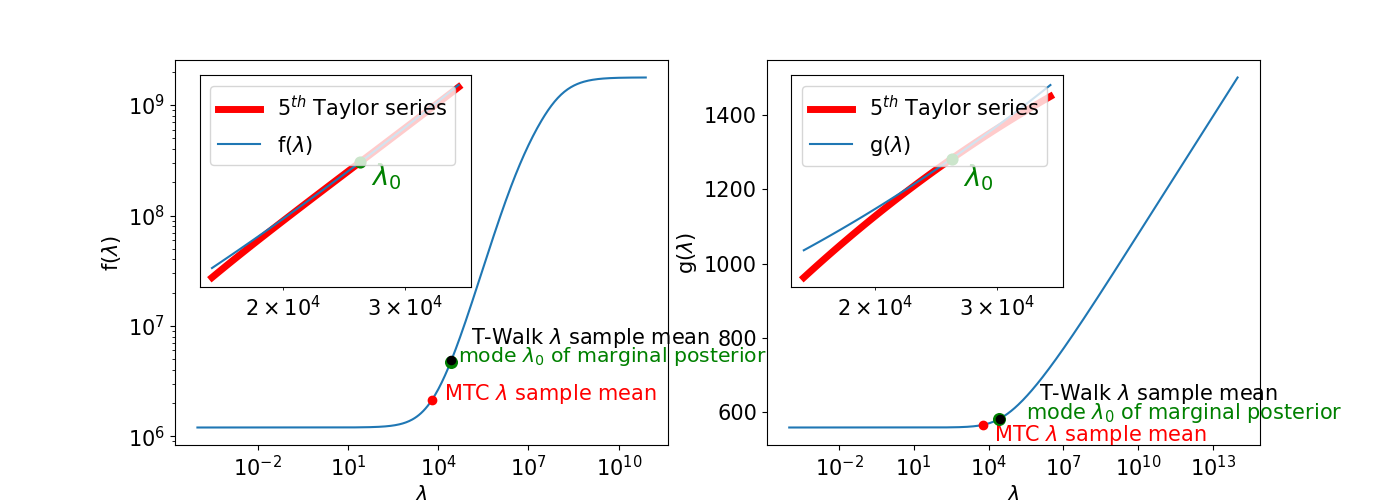
\includegraphics[width=1\textwidth]{OxThesis-master/figures/f_and_g.png} 
\caption[Plotting $f(\lambda)$ and $g(\lambda)$ for a large range of $\lambda$ to characterize the marginal posterior distribution.]{\textbf{Plotting $f(\lambda)$, Eq. \ref{eq:gtay}, and $g(\lambda)$, Eq.m \ref{eq:gtay}, for a large range of $\lambda$ to characterize the marginal posterior distribution.}
We included the samples mean of the MTC-Sampling (red) and T-walk algorithm (black) \cite{}. In the upper left corner of each figure, we plotted the Taylor series (red) of $f(\lambda)$ and $g(\lambda)$ around the mode of the marginal posterior $\pi(\delta_0, \gamma_0 | \bm{y})$, where $\lambda_0 = \delta_0 / \gamma_0 $. To display the Taylor series we computed up to the fifth derivatives of each function. Note that we usually only focus on a small range of $\lambda$ compared to the here shown range.}
\label{fig:fandg}
\end{figure}
In doing so we set up a specific forward model, in which we specify the number of layers and the number of measurements, to determine the Equations \ref{eq:gammaPrior} and \ref{eq:lamPrior}.
We measure $m = 105$ times equally spaced in between the tangent heights of $2$km and $100$km.
We were given data of $n = 47$ Ozone layers so that the Ozone concentration is zero below 5km and above 90km, as indicated in Figure \ref{fig:forModel}.
We stimulated white noise with a standard deviation of 1\% of the maximum value of data and plotted this in golden color in see Figure \ref{fig:RecRes}.
We calculate the function $f(\lambda)$ and $g(\lambda)$ by using the linear solver \textit{gmres} of the \textit{scipy.sparse.linalg} package in \textit{Python}.
We use the solver to compute the matrix multiplication of $\bm{B}^{-1}\bm{L}$ and $\bm{B}^{-1} \bm{F}^T \bm{y}$, where we set the tolerances for convergence to $10^{-7}$ and repeat the process after 25 iterations.
For a large range of $\lambda$ we plotted $f(\lambda)$ and $g(\lambda)$ in Figure \ref{fig:fandg} and include some results of the sampling process such as sample mean of the MTC-Sampler in red and of the T-Walk algorithm in black.
The top left corner of each figure shows the Taylor approximation around the mode of the marginal posterior distribution in red underneath the original function in blue.

\begin{figure}[thb]
 \begin{subfigure}{0.5\textwidth}
     \centering
     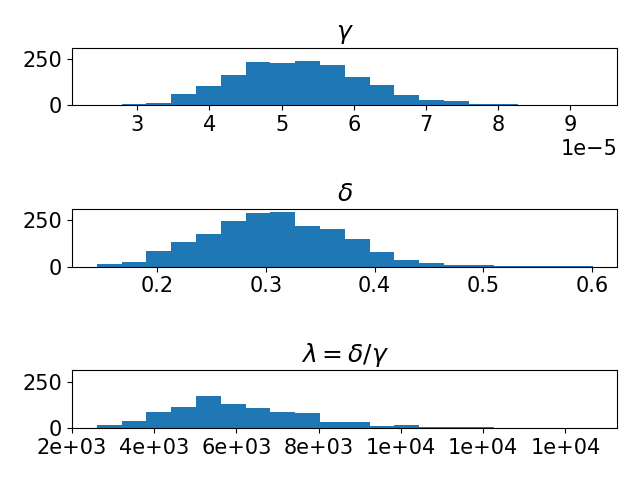
\includegraphics[width=\textwidth]{OxThesis-master/figures/HistoResults.png}
     \caption{}
     \label{fig:MTCHisto}
 \end{subfigure}
 \hfill
 \begin{subfigure}{0.5\textwidth}
     \centering
     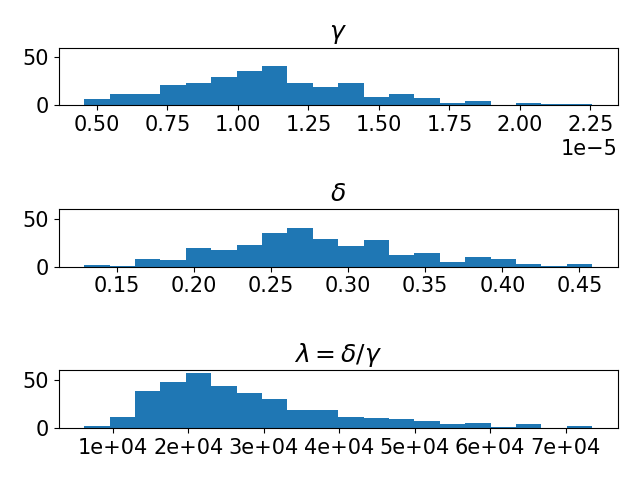
\includegraphics[width=\textwidth]{OxThesis-master/figures/PyTWalkHistoResults.png}
      \caption{}
     \label{fig:TWalkHisto}
 \end{subfigure}
\caption[Sampling Results of the MTC-Sampler and the T-Walk algorithm \ref{fig:TWalkHisto}]{\textbf{Sampling Results of the MTC-Sampler \ref{fig:MTCHisto} and the T-Walk algorithm \ref{fig:TWalkHisto}.} The histograms present independent samples of the marginal posterior distribution according to their integrated Auto-correlation time $\tau_{int}$.
Using the \textit{UWerr.m} function by U. Wolff we calculate integrated auto-correlation times of $\tau_{\text{int}, \text{MTC}, \gamma} = 5.4$, $\tau_{\text{int}, \text{MTC}, \delta} = 4.9$ and $\tau_{\text{int}, \text{MTC}, \lambda}= 10.2$ when utilizing the MTC-Sampler with an acceptance rate of 0.34 \cite{Uwerr}.
Running the T-Walk algorithm we obtain following auto-correlation times: $\tau_{\text{int}, \text{T-walk}, \gamma} = 34.1$, $\tau_{\text{int}, \text{T-walk}, \delta} = 34.5$ and $\tau_{\text{int}, \text{T-walk}, \lambda}= 27.5$, with an acceptance rate of 0.42.}
\label{fig:histRes}
\end{figure}
Next, we found the mode at $(\gamma_0, \delta_0) = (1 \times 10^{-5}, 0.26)$ of the marginal posterior distribution by using the \textit{optimize.fmin} function from the \textit{scipy} package in \textit{Python}.
In Figure \ref{fig:fandg} this mode is indicated in green and is the value where we initialize our Markov chain.
We use a normal proposal distribution so that $\lambda' | \lambda \sim \mathcal{N}(\lambda| w^2_{\lambda})$ and draw $10^4$ samples of the marginal posterior distribution, with a burn in period of 50 samples.
We tune variance of the proposal distribution so that the acceptance ratio is between 0.25 and 0.5, and set $w_{\lambda} = 5\times 10^3$.
After calculating the auto-correlation times with \textit{MATLAB} function \textit{UWerr.m} by Ulli Wolff we calculate integrated auto-correlation times \cite{Uwerr}.
Note that we use two times the values of the output of that function, as indicated in \cite{fox2016fast}.
Given the integrated auto-correlation times, we can generate independent samples of the marginal posterior distribution $\pi(\lambda, \gamma | \bm{y})$, see Figure \ref{fig:histRes}.
The integrated auto-correlation times of the MTC-Sampler are: $\tau_{\text{int}, \text{MTC}, \gamma} = 5.4$, $\tau_{\text{int}, \text{MTC}, \delta} = 4.9$ and $\tau_{\text{int}, \text{MTC}, \lambda}= 10.2$.
This is significantly lower compared to the T-Walk algorithm, which needs more than 34 samples to draw two independent hyper-parameter values.
\mccorrect{We indicated the sample mean in Figure} \ref{fig:fandg}\mccorrect{and would like to point out that the T-walk algorithm hits the precalculated mode of the marginal posterior quite accurately.
The MTC-Sampler seems to have a bigger $\gamma$ sample mean compared to the true value.
This reduces the value of $\lambda$ from around $2 \times 10^5$ to $5 \times 10^4$.}

\begin{figure}[htb]
\centering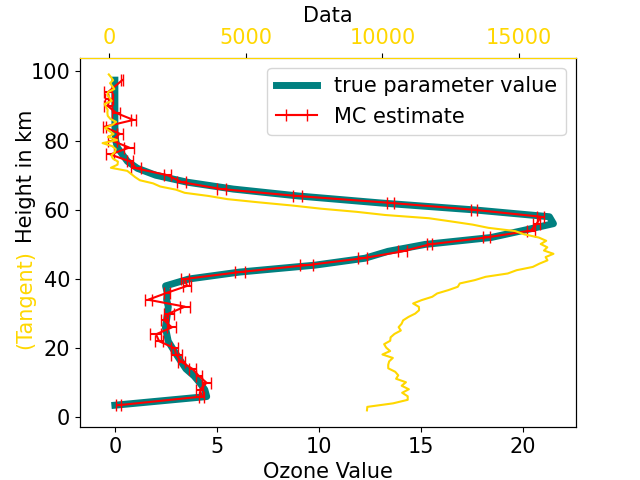
\includegraphics[width=0.7\textwidth]{OxThesis-master/figures/FirstRecRes.png} 
\caption[Randomize then Optimize (RTO) method to recover the Ozone profile in dependency of the height.]{\textbf{Randomize then Optimize (RTO) method to recover the Ozone profile in dependency of the height.} Here we plotted the mean of 10 posterior samples and their variance in red. We draw hyper-parameter samples according to the samples seen in Figure \ref{fig:MTCHisto}. In green, we displayed the true Ozone profile $\bm{x}$.
We show the data $\bm{y}$ including noise in golden for each tangent height.}
\label{fig:RecRes}
\end{figure}
Given the samples obtained by the MTC-Sampler, see Figure \ref{fig:MTCHisto}, we draw hyper-parameters from the marginal posterior accordingly.
The Randomize then Optimize (RTO) method allows us to compute parameter samples from the full posterior $\pi(\bm{x},\lambda, \gamma|\bm{y})$.
We solve Equation \ref{eq:RTOapplied} for 10 independent hyper-parameter samples to obtain 10 parameter samples.
We plot the results in Figure \ref{fig:RecRes}, where the red line indicates the sample mean including the sample variance.
The results match up well with the true Ozone profile plotted in green.
We included the data $\bm{y}$ in dependency of the tangent height in golden color.

%######################### ideas #####################

% The main goal of this thesis is to apply the introduced samplers to atmospheric trace gas measurements.
% Here we introduce a atmospheric model first a linear model and then raise complexity for the non-linear case.
% The model is suitable to describe a measurement process for a LIMB-Sounder

% \mccorrect{Maybe at the beginning.. or mention at the beginning that this is the motivation for this work.. speed up sampling.. can we deliver real time data?}

% \begin{itemize}
%     \item figure of atmosphere
%     \item Limb sounder - basic principles
%     \item linear model
%     \item non linear model
% \end{itemize}



% -how to sep up a model
% - scaling of the froward map and scaling
% -hyperparameter
% -sample from hyperpriors




%% APPENDICES %% 
% Starts lettered appendices, adds a heading in table of contents, and adds a
%    page that just says "Appendices" to signal the end of your main text.
\startappendices
% Add or remove any appendices you'd like here:
\chapter{Posterior of Bayesian Hierachical model}
\label{ap:bayesian}
Here we show how to obtain the posterior covariance and mean of our hierarchical Bayesian model in \ref{eq:prior} - \ref{eq:post}.
We do not consider the hyper-parameters and start with the joint probaility distribution of $(\bm{x}^T,\bm{y}^T)^T$, where $\bm{x} \in \mathcal{X}$ and $\bm{y} \in \mathcal{Y}$ do not intersect.
For more details we refer to Chapter 2 in \cite{bishop2006pattern} and to the book of Rue and Held \cite{rue2005gaussian}.

The exponent of the normal Gaussian can be rewritten into:
\begin{align}
\label{eq:gauss}
    -\frac{1}{2}(\bm{x} - \bm{\mu})^T \bm{Q} (\bm{x} - \bm{\mu}) = - \frac{1}{2} \bm{x}^T \bm{Q} \bm{x} + \bm{x}^T \bm{Q} \bm{\mu} + \text{const.}
\end{align}
We like to bring the joint distribution into a similar form so that we can compare the linear and second order terms and find the precision matrix and mean of the joint distribution.


In general the joint distribution to find the experssino for the postiror dostrbution

We can express this posterior through the likelihood and prior probability by Bayesian theorem, with a constant and positive normalization constant:
\begin{equation}
    \pi(\bm{x} |\bm{y}) \propto \pi( \bm{y} | \bm{x} )  \pi(\bm{x} )
\end{equation}
Taking the logarithmic function of this formulation we can find an expression for the the posterior covariance, with the $\text{Var}(\bm{x}) = \bm{Q_x}^{-1}$ and $\text{Var}(\bm{y}) = \bm{Q_y}^{-1}$.
\begin{align}
\ln{\pi(\bm{x|y})} \propto&  \ln{ \pi( \bm{y} | \bm{x} ) } + \ln{\pi( \bm{x} ) }\\
=& - \frac{1}{2} (\bm{x} - \bm{\mu} )^T \bm{Q_x} (\bm{x} - \bm{\mu} ) - \frac{1}{2} (\bm{y} - \bm{Ax} )^T \bm{Q_y} (\bm{y} - \bm{Ax} )    \\
=& - \frac{1}{2} \bigg[ \bm{x}^T \big[ \bm{Q_x} + \bm{A}^T \bm{Q_y} \bm{A} \big] \bm{x}  + \bm{x}^T \big[ - \bm{A}^T \bm{Q_y} \big] \bm{y} \\
&+ \bm{y}^T \big[ - \bm{Q_y A} \big] \bm{x} + \bm{y}^T \big[ \bm{Q_y} \big] \bm{y} - 2 \bm{x}^T \bm{Q_x \mu }  \bigg] + \text{const.}
\end{align}

Hence we deal with a Gaussian distribution, we consider second order terms only and rearrange to the precision matrix.
\begin{align}
    &- \frac{1}{2} \begin{bmatrix}
        \bm{x}^T \big[ \bm{Q_x} + \bm{F}^T \bm{Q_y} \bm{F} \big]  + \bm{y}^T \big[ - \bm{Q_y F} \big] & \bm{y}^T \big[ \bm{Q_y} \big] + \bm{x}^T \big[ - \bm{F}^T \bm{Q_y} \big] 
    \end{bmatrix}  \begin{bmatrix}
        \bm{x} \\ \bm{y}
    \end{bmatrix} \\
    =& \begin{bmatrix}
        \bm{x}^T & \bm{y}^T
    \end{bmatrix} 
    \underbrace{\begin{bmatrix}
        \bm{Q}_x + \bm{F}^T \bm{Q}_y \bm{F} & - \bm{F}^T \bm{Q}_y \\
        -\bm{Q}_y \bm{F} & \bm{Q}_y
    \end{bmatrix}}_\text{precision matrix} \begin{bmatrix}
        \bm{x} \\ \bm{y}
    \end{bmatrix} 
\end{align}
We denote the precision matrix of the joint field as:
\begin{align}
    \bm{Q}_{xy} = \begin{bmatrix}
        \bm{Q}_{aa} & \bm{Q}_{ab} \\
        \bm{Q}_{ba} & \bm{Q}_{bb}
    \end{bmatrix} = 
    \begin{bmatrix}
        \bm{Q}_x + \bm{F}^T \bm{Q}_y \bm{F} & - \bm{F}^T \bm{Q}_y \\
        -\bm{Q}_y \bm{F} & \bm{Q}_y
    \end{bmatrix}
\end{align}

The mean is defined through the linear term.
\begin{align}
    \frac{- 2 \bm{x}^T \bm{Q_x \mu } }{-2} = \begin{bmatrix}
        \bm{x}^T & 0
    \end{bmatrix} \begin{bmatrix}
        \bm{Q_x \mu}\\ 0
    \end{bmatrix} 
    \end{align} 
Comparing to the linear term of Equation \ref{eq:gauss} we can formulate an expression for the joint mean:
    \begin{align}
    \Rightarrow \bm{\mu_{xy}} = \bm{Q}_{\bm{x}\bm{y}}^{-1}   \begin{bmatrix}
        \bm{Q_x \mu}\\ 0
    \end{bmatrix}
\end{align}
The mean of the conditional distribution $\bm{x}|\bm{y}$ is given by:
\begin{align}
\bm{\mu}_{\bm{x}|\bm{y}} &= \bm{\mu}_{\bm{x}} + \bm{Q}^{-1}_{ba} \bm{Q}_{ab} (\bm{x} - \bm{\mu}_{\bm{y}}) \\
\bm{\mu}_{\bm{x}|\bm{y}} &= \bm{\mu} +  ( \bm{Q}_x + \bm{F}^T \bm{Q}_y \bm{F} )^{-1} \bm{F}^T \bm{Q}_y ( \bm{x} - \bm{F \mu} ) \, ,
\end{align}
and the covariance of $\bm{x}|\bm{y}$ is given by:
\begin{align}
   \bm{Q}_{\bm{x}|\bm{y}} =  \bm{Q}_{aa} = \bm{Q}_x + \bm{F}^T \bm{Q}_y \bm{F} \, ,
\end{align}
as illustrated through Theorem 2.5 in \cite{rue2005gaussian}.


\chapter{Convergence of the Metropolis-Hastings}
\label{ap:MetroHast}

If we show that the detailed balance condition holds and that the state space is irreducible and aperiodic under the transition matrix $\bm{P}$, we generate a Markov chain with a unique stationary distribution proportional to $\pi (\bm{x} , \bm{\theta} | \bm{y})$.
Since the posterior is strictly positive $\pi (\bm{x} , \bm{\theta} | \bm{y}) \geq 0$ on the finite state space $\Omega(\mathcal{X},\mathcal{\theta})$ the generated chain is irreducable.
Further, it is possible to reject any proposed state and stay in the current state, which leads to aperiodicity.
The detailed balance holds for the case that $\bm{j} = \bm{i}$, but if $\bm{j} \neq \bm{i}$ it is not trivial.
In case we accept $\{ \bm{x}, \bm{\theta} \}^{(n+1)} = \bm{j}$ as the new state we have $ \pi(\bm{j} | \bm{y})  g(\bm{i}|\bm{j})> \pi(\bm{i} | \bm{y})  g(\bm{j}|\bm{i})$.
This gives us $\alpha(\bm{j}|\bm{i}) = 1$ and $\alpha(\bm{i}|\bm{j}) = \frac{\pi_{\bm{i}} g(\bm{j}|\bm{i})}{\pi_{\bm{j}} g(\bm{i}|\bm{j})}$ and satisfies the detailed balance:
\begin{align*}
    \cancel{\pi_{\bm{j}}}  \frac{\pi_{\bm{i}}}{\cancel{\pi_{\bm{j}}}} g(\bm{j}|\bm{i}) &= \pi_{\bm{i}} g(\bm{j}|\bm{i}) \quad .
\end{align*}
If $ \pi(\bm{j} | \bm{y})  g(\bm{i}|\bm{j}) < \pi(\bm{i} | \bm{y})  g(\bm{j}|\bm{i})$ then $\alpha(\bm{i}|\bm{j}) = 1$
and $\alpha(\bm{j}|\bm{i}) = \frac{\pi_{\bm{j}} g(\bm{i}|\bm{j})}{\pi_{\bm{i}} g(\bm{j}|\bm{i})}$, this satisfies the detailed balance as well.

In conclusion the Metropolis-Hastings algorithm samples from a unique distribution proportional to the posterior distribution. 

\chapter{Randomize then Optimize - RTO}
\label{ap:RTO}

\begin{align}
    \pi(\bm{x}|\bm{y}, \bm{\theta} ) &\propto \pi(\bm{y} | \bm{x} , \bm{\theta} ) \pi(\bm{x}| \bm{\theta}) \\
   &\propto \exp \Big[  ( \bm{F x} - \bm{y})^T \bm{\Sigma}^{-1}( \bm{F x} - \bm{y}) + (\bm{x} -\bm{\mu} )^T \bm{Q} (\bm{x} -\bm{\mu})\Big] \\
   &= \exp  \lVert \hat{\bm{F}} \bm{x} - \hat{\bm{y}} \rVert^2 
\end{align}
where 
\begin{align}
\hat{\bm{F}} = 
    \begin{bmatrix}
         \bm{\Sigma}^{-1/2} \bm{F}\\
    \bm{Q}^{1/2}
    \end{bmatrix} \, , \quad \hat{\bm{y}} = 
    \begin{bmatrix}
        \bm{\Sigma}^{-1/2} \bm{y} \\
        \bm{Q}^{1/2}\bm{\mu}
    \end{bmatrix}
\end{align}

One sample from the posterior can be computed by minimizing the following with respect to $\bm{x}$
\begin{align}
    \bm{x} = \arg \min_{\hat{\bm{x}}} \lVert \hat{\bm{F}} \hat{\bm{x}} - ( \hat{\bm{y}} + \bm{\eta} ) \rVert^2 , \quad \bm{\eta} \sim \mathcal{N}(\bm{0}, \mathbf{I})
\end{align}

We can solve this and rewrite to
\begin{align}
    \frac{\partial}{\partial \bm{x} }  \big[   (\hat{\bm{F}} \bm{x} - ( \hat{\bm{y}} + \bm{\eta} )^T (\hat{\bm{F}} \bm{x} - ( \hat{\bm{y}} + \bm{\eta} ) \big] &= 0 \\
    \Leftrightarrow \bm{x}^T \hat{\bm{F}}^T  \hat{\bm{F}} + \hat{\bm{F}}^T \hat{\bm{F}} \bm{x} -  \hat{\bm{F}}^T ( \hat{\bm{y}} + \bm{\eta} )- ( \hat{\bm{y}} + \bm{\eta} )^T  \hat{\bm{F}} \bm{x}  &= 0
\end{align}
We can argue through the symmetry of the inner product that and the symmetry of the precision matrix
\begin{align}
    \hat{\bm{F}}^T \hat{\bm{F}} \bm{x} &= \hat{\bm{F}}^T ( \hat{\bm{y}} - \bm{\eta}) \\
    \Leftrightarrow  (\bm{F}^T \bm{Q_y} \bm{F}+
    \bm{Q} ) \bm{x} &= \bm{F}^T \bm{Q_y} \bm{y} +  \bm{Q} \bm{\mu} - \hat{\bm{F}}^T  \bm{\eta}  
\end{align}
If we substitute $ - \hat{\bm{F}}^T  \bm{\eta}  = \bm{v}_1 + \bm{v}_2$ we end up with 
\begin{align}
    (\bm{F}^T \bm{\Sigma}^{-1} \bm{F}+
    \bm{Q} ) \bm{x} &= \bm{F}^T \bm{\Sigma}^{-1} \bm{y} +  \bm{Q} \bm{\mu} + \bm{v}_1 + \bm{v}_2
\end{align}
where $\bm{v}_1 \sim \mathcal{N}(\bm{0}, \bm{F}^T \bm{\Sigma}^{-1} \bm{F}) $ and $\bm{v}_2 \sim \mathcal{N}(\bm{0}, \bm{Q} )$ are independent random variables.
mayeb introduce... $x^2$ time nomral variubale


\chapter{Inverting Matrices - QR factorization}


\chapter{Taylor expansion of  $g(\lambda)$}
\label{ap:taylor}
We Taylor expand the function $g(\lambda)$ around $\lambda = \lambda'  - \Delta \lambda$
\begin{align}
    g(\lambda) = \ln \det \underbrace{(\bm{F}^T  \bm{F} + \lambda \bm{L})}_{\bm{B}}
\end{align}
\begin{align}
       g(\lambda') -    g(\lambda) &=  \ln \det ( \bm{F}^T  \bm{F} + \lambda' \bm{L}) -  \ln \det (\bm{F}^T  \bm{F} + \lambda \bm{L}) \\
    &=  \ln \det \Bigg[ \frac{(\bm{F}^T  \bm{F} + (\lambda + \Delta \lambda) \bm{L}) }{ ( \bm{F}^T  \bm{F} + \lambda \bm{L}) } \Bigg]  \\
       &=  \ln \det \Bigg[ 1 + \frac{ \Delta \lambda \bm{L} }{ \bm{B} } \Bigg]\\
       & = \sum_{r = 1}^{\infty} \frac{(-1)^{r+1}}{r !}\text{tr} (   (\bm{B}^{-1}  \bm{L} )^r  )  (\Delta \lambda)^r
\end{align}, where we use the identity from \cite{gohberg2012traces} at page 29.
So the derivatives of $g(\lambda)$ are:
\begin{align}
    g^{(r)} ( \lambda) =&  (-1)^{r+1} \, \text{tr} \big( (\bm{B}^{-1}\bm{ L })^r \big)\\
\approx& (-1)^{r+1} \sum^p_{k=1} \bm{z_k}^T (\bm{B}^{-1} \bm{L} )^r \bm{z_k}  
\end{align} 
Here we use a Monte Carlo estimate and draw $p$ vectors $\bm{z_k} \in \mathbb{R}^n $, where each vector element $z_i \overset{\text{i.i.d.}}{\sim} \mathcal{U} ( \{ -1, 1 \} )$ and $i = 1 , \dots, n$.

\chapter{Radiation transfer and absorption line shape}
\label{ap:RTE}


\chapter{whispering gallery resonator}
\label{ap:resonator}


\begin{figure}
\centering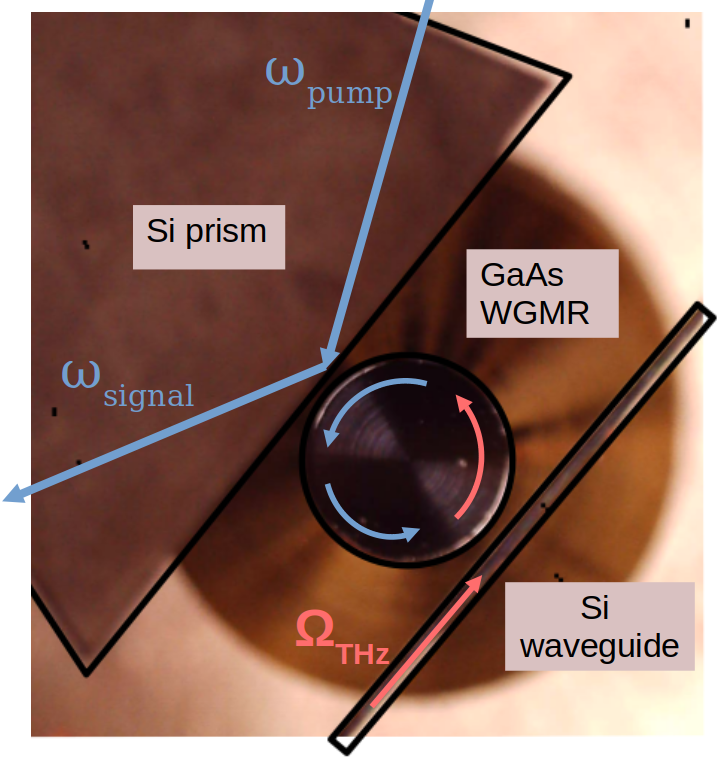
\includegraphics[width=0.7\textwidth]{GaAs_setup4.png} 
\caption[whispering gallery resonator]{whispering gallery resonator}
\label{fig:GaAsRes}
\end{figure}


%%%%% REFERENCES\\


{\renewcommand*\MakeUppercase[1]{#1}%
\printbibliography[heading=bibintoc,title={\bibtitle}]}


\end{document}
